\documentclass[a4paper,11pt]{article}
% inputenc 제거 — XeLaTeX에서는 불필요하고 충돌 유발
\usepackage{kotex}
\usepackage[margin=2.5cm]{geometry}
\usepackage{microtype}
\usepackage{hyperref}
\usepackage{booktabs}
\usepackage{graphicx}
\usepackage{amsmath,amsfonts}
\usepackage{multirow}
\usepackage{xcolor}
\usepackage{enumitem}
\usepackage{float}
\usepackage{natbib}
\DeclareMathOperator*{\argmax}{arg\,max}

\title{멀티 에이전트 LLM 시스템은 언제 멈춰야 하는가? \\ 토폴로지 인식 종료 역학}
\author{Anonymous Authors}
\date{}

\begin{document}

\maketitle

\begin{abstract}
멀티 에이전트 LLM 시스템은 언제 작업을 멈춰야 하는가? 멀티 에이전트 협업이 추론 시점 연산(inference-time compute) 확장의 주요 메커니즘으로 부상하는 가운데, 치명적 공백이 존재한다: 종료 기준이 토폴로지에 무관하게 적용되어, 에이전트 조정 방식과 무관하게 동일한 고정 턴 한도가 쓰이며, 출력 품질을 오히려 저하시키는 구성에 연산을 낭비한다. 14개 조정 패턴에 걸친 2,200회 이상의 통제 실험을 통해, 현행 가정을 뒤집는 세 가지 발견을 제시한다. 첫째, \emph{에이전트가 많아도 비용이 줄 수 있다}: 탈중앙 라우팅이 대형 순차 체인을 능가하며, 시스템 규모가 아닌 토폴로지가 비용을 결정한다. 둘째, \emph{추가 연산이 해를 끼칠 수 있다}: 멀티 에이전트 토론은 첫 라운드 이후 품질이 저하되며, 우리의 하이브리드 한계 효용 기준은 품질 손실 없이 낭비된 토큰의 78\%를 회수한다. 셋째, \emph{난이도가 토폴로지를 $7.8\times$ 압도한다}: 대부분의 모델에서 단일 에이전트가 쉬운 과제에서 모든 멀티 에이전트 시스템을 능가하며, 피드백 협업은 능력 있는 모델에서만 어려운 과제에 유효하다. 다수 모델과 제공자에 걸쳐 검증된---역대 최대 규모의 교차 토폴로지 종료 연구---이 결과는, 실무자가 \emph{어떤} 토폴로지를 쓸지보다 멀티 에이전트 시스템을 \emph{쓸 것인지} 여부를 먼저 결정해야 함을 확립한다. 실험 프레임워크와 토폴로지 인식 설계 가이드라인을 공개한다.
\end{abstract}

%% ========================================================
\section{서론}
%% ========================================================

\subsection{왜 종료가 중요한가}

AutoGen (Wu et al., 2023), CrewAI, LangGraph 등의 프레임워크를 통한 LLM 기반 멀티 에이전트 시스템의 배포가 빠르게 확대되고 있다. 이들 시스템이 확장됨에 따라 치명적 비용 문제가 부상한다: 멀티 에이전트 협업은 단일 에이전트 대비 3--17$\times$의 토큰 오버헤드를 유발하며, 부적절한 종료 기준은 출력 품질을 오히려 저하시키는 구성에서 최대 78\%의 연산을 낭비한다. 그러나 \textbf{이 시스템들이 언제 멈춰야 하는가}라는 근본적 질문은 아직 탐구되지 않았다.

이 질문은 \emph{추론 시점 연산 스케일링(inference-time compute scaling)}과 직결된다: 멀티 에이전트 협업은 구조화된 테스트 타임 연산 배분이며, 최적 종료 시점은 추가 연산이 체감 수익을 낳는 포화 경계를 정의한다.

현행 관행은 토폴로지와 무관하게 획일적으로 적용되는 원시적 종료 기준에 의존한다:
\begin{enumerate}[label=(\roman*)]
    \item 고정 최대 턴 수
    \item 키워드 감지 (예: ``TERMINATE'')
    \item 외부 타임아웃 신호
\end{enumerate}

이러한 휴리스틱은 핵심 통찰을 무시한다: \textbf{최적 종료 시점은 에이전트의 조정 방식에 근본적으로 의존한다.} 사실 확인 질문을 푸는 2-에이전트 라운드 로빈 팀은 2턴 만에 충분한 답을 낼 수 있으나, 3-에이전트 토론 팀은 합의에 도달하기 위해 여러 교환 라운드가 필요할 수 있다. 동일한 종료 로직을 양쪽에 적용하면 필연적으로 조기 종료(품질 손실) 또는 불필요한 계산(자원 낭비)이 발생한다.

이 불일치를 \textbf{종료 후회(termination regret)}라 정의한다---팀이 실제로 멈춘 시점과 품질-비용 트레이드오프를 최적화하기 위해 멈춰야 했던 시점 사이의 차이. 세 가지 구체적 시나리오를 고려하자:

\begin{itemize}
    \item \textbf{과잉 종료(Over-termination):} 토론 팀이 모든 에이전트가 합의한 이후에도 4라운드를 더 교환하며, 품질 개선 없이 토큰을 소비한다.
    \item \textbf{과소 종료(Under-termination):} 순차 파이프라인이 첫 단계의 초안 출력 후 멈추며, 사실 오류를 수정했을 정제 단계에 도달하지 못한다.
    \item \textbf{토폴로지 불일치(Topology mismatch):} 선택자(selector) 기반 팀에 고정 순차 패턴용으로 보정된 max-turn 종료를 적용하여, 라우팅 에이전트가 적절한 전문가를 참조하기 전에 차단한다.
\end{itemize}

\subsection{우리의 접근법}

이 문제를 체계적으로 조사하기 위해, 역대 최대 규모의 교차 토폴로지 종료 연구를 수행한다: 6개 토폴로지 범주에 걸친 14개 조정 패턴에서 2,200회 이상의 통제 실험을 수행하며, 효율성 측정에서 품질 추적, 수렴 감지, 오류 귀인, 적응적 종료, 비용 예측, 난이도 상호작용에 이르는 7개 실험으로 구성된다. 오픈웨이트 모델을 포함한 다수 제공자의 다수 모델에 걸쳐 일반화 가능성을 검증한다.

\subsection{연구 질문}

본 연구의 7개 연구 질문:

\textbf{RQ1}: 종료 역학(지속 시간, 턴 수, 토큰 소비)은 조정 토폴로지에 따라 어떻게 다른가? (실험 01)

\textbf{RQ2}: 턴별 품질 궤적을 측정하고 최적 종료 시점을 사후 식별하여 종료 후회를 감지할 수 있는가? (실험 02)

\textbf{RQ3}: 구조화 피드백 패턴(반성, 토론)이 적응적 종료에 활용 가능한 측정 가능한 수렴 신호를 나타내는가? (실험 03)

\textbf{RQ4}: 서로 다른 토폴로지가 출력에서 특징적인 오류 패턴을 생성하는가? (실험 04)

\textbf{RQ5}: 한계 효용(marginal utility) $\Delta U(t) = \Delta Q(t) - \lambda \cdot \Delta C(t)$가 0으로 수렴하는 최적 정지점이 존재하며, 이를 활용한 적응적 종료가 고정 기준 대비 파레토 프론티어를 개선할 수 있는가? (실험 05)

\textbf{RQ6}: 사전 실행 토폴로지 특성이 런타임 비용을 예측할 수 있으며, 어떤 특성이 가장 예측력이 높은가? (실험 06)

\textbf{RQ7}: 과제 난이도가 최적 토폴로지 선택을 조절하며, 토폴로지 간 품질 격차가 난이도에 따라 확대 또는 축소되는가? (실험 07)

\subsection{기여}

본 연구의 7가지 기여:

\begin{enumerate}
    \item \textbf{교차 토폴로지 종료 연구.} 통합 프레임워크 내에서 6개 토폴로지 범주에 걸친 14가지 조정 패턴의 종료 행동을 최초로 체계 비교한다. 선행 연구는 최대 2--3개 패턴만 비교했다 (Cemri et al., 2025; Hu et al., 2025).

    \item \textbf{종료 후회 지표.} G-Eval (Liu et al., 2023) 스코어링을 각 에이전트 턴에 적용하여 품질 궤적을 구축하고, 품질이 정점에 도달한 시점과 팀이 종료한 시점을 정밀 비교하는 사후 분석법을 도입한다. 이를 통해 피드백 패턴의 체계적 과잉 계산과 고정 순차 패턴의 과소 계산을 밝힌다.

    \item \textbf{주장 수준 수렴 감지.} 토론 안정성 감지를 위한 Hu et al. (2025)의 KS-검정 접근법을 확장하여, 전체 13개 토폴로지에서 턴 간 주장 수준 의미적 안정성을 추적하고, 수렴 신호가 토폴로지 의존적임을 밝힌다.

    \item \textbf{패턴별 오류 분류 체계.} MAST 오류 범주(환각, 불완전성, 불일치)와 정렬하여, 오류 유형 분포가 토폴로지 특성과 상관함을 보인다: 순차 패턴은 불완전성 오류를, 피드백 패턴은 충돌 수정으로 인한 불일치 오류를 더 많이 생성한다.

    \item \textbf{한계 효용 진단 프레임워크와 ``부정적 결과''의 가치.} $\Delta U(t) = \Delta Q(t) - \lambda \cdot \Delta C(t)$를 새로운 최적화 알고리즘이 아닌, 두 가지 기여를 동시에 생산하는 원칙적 진단 렌즈로 도입한다. \emph{긍정적 기여}: $\Delta U$가 키워드 종료가 실패하는 특정 토폴로지 유형(탈중앙 핸드오프/B2)을 식별하여, swm4에서 70\% 비용 절감을 달성한다---선행 연구에 없던 타겟된 권고. \emph{부정적 결과 기여}: 800회 통제 실험에서 정교한 적응적 종료가 대부분의 배포에서 불필요함을 입증한다. 이 ``부정적 결과''---키워드 종료가 7/8 토폴로지에서 거의 최적---는 기존 실무자 휴리스틱을 정량적 증거로 검증한다는 점에서 유의한 실용적 가치를 가진다. $\Delta U(t) \to 0$ 수식은 품질 포화(반복 정제의 보편적 속성)를 활용하여 $\lambda$ 선택과 무관하게 토폴로지 의존적 수렴 속도 측정(1.1--2.4턴)을 가능하게 한다. 핵심 통찰은 수식 자체가 아니라, 해당 수식을 13개 토폴로지에 최초로 체계적으로 적용했을 때 \emph{밝혀지는 것}이다.

    \item \textbf{토폴로지 기반 비용 예측.} 사전 실행 토폴로지 특성(에이전트 수, 최대 메시지 수, 패턴 범주, 상호작용 항 \texttt{agent\_count $\times$ max\_messages})이 런타임 토큰 소비를 중간 정확도(Random Forest $R^2=0.54$, 5-fold CV)로 예측함을 입증한다. 상호작용 항이 가장 강력한 예측 변수로 나타나, 실행 전 비용 추정의 원칙적 기반을 제공한다. 나머지 ${\sim}46\%$의 분산은 과제 내용 복잡도에 기인하며, 토폴로지 특성만의 예측 한계를 정직하게 규정한다.

    \item \textbf{모델 능력 조건부 난이도 상호작용.} 6개 모델(Haiku~4.5, Opus~4.6, GPT-4o-mini, GPT-5.4, Grok~3~Mini, Gemini-2.0-Flash)에 걸친 743회 실행에서 Solo가 쉬운 과제에서 5/6 모델에서 최적이며, 피드백 협업은 능력 있는 기반 모델에서만 보통/어려운 과제에서 이점을 보인다 ($\eta^{2}_{H}=0.364$ vs $\eta^{2}_{H}=0.046$).
\end{enumerate}

\subsection{범위와 포지셔닝}

본 연구는 토폴로지 인식 종료를 위한 실증적 토대를 제공하며, 후속 알고리즘 개발의 방향을 결정하는 체계적 벤치마크(예: NLU의 GLUE, 언어 모델의 HELM)의 전통을 따른다. 기존 연구에서 단일 통제된 프레임워크 내에서 2--3개 이상의 토폴로지에 걸쳐 종료 역학을 체계적으로 비교한 선행 연구는 없다. 14개 패턴, 7개 실험, 2,200회 이상의 실행을 통해, 어떤 토폴로지에 적응적 종료가 필요하고 어떤 토폴로지에는 필요하지 않은지---그리고 그 이유를---확립하며, 이는 실무자의 설계 결정과 향후 알고리즘 연구 모두에 직접적으로 기여한다.

\subsection{논문 구성}

2절에서 관련 연구를 조사하고, 3절에서 13가지 조정 패턴의 분류 체계와 실험 프레임워크를 기술한다. 4절에서 7개 상호 연결 실험의 결과를 제시하고, 5절에서 시사점과 한계를 논의하며, 6절에서 결론을 맺는다.

%% ========================================================
\section{배경 및 관련 연구}
%% ========================================================

\subsection{멀티 에이전트 조정 토폴로지}

멀티 에이전트 LLM 시스템은 다양한 조정 전략을 활용한다. 본 연구는 고전적 MAS(Multi-Agent Systems) 토폴로지 이론 (Masterman et al., 2025)에 기반하여 13개 패턴을 \textbf{5개 범주}로 조직한다 (그림~\ref{fig:taxonomy}). Masterman et al.은 MAS의 3대 정규 토폴로지를 \textbf{체인(Chain)}, \textbf{스타(Star/Hub-and-Spoke)}, \textbf{메시(Mesh/Swarm)}로 분류한다. 본 연구는 이에 피드백 루프와 복합 아키텍처를 추가하여 다음과 같이 확장한다:

\begin{figure}[H]
    \centering
    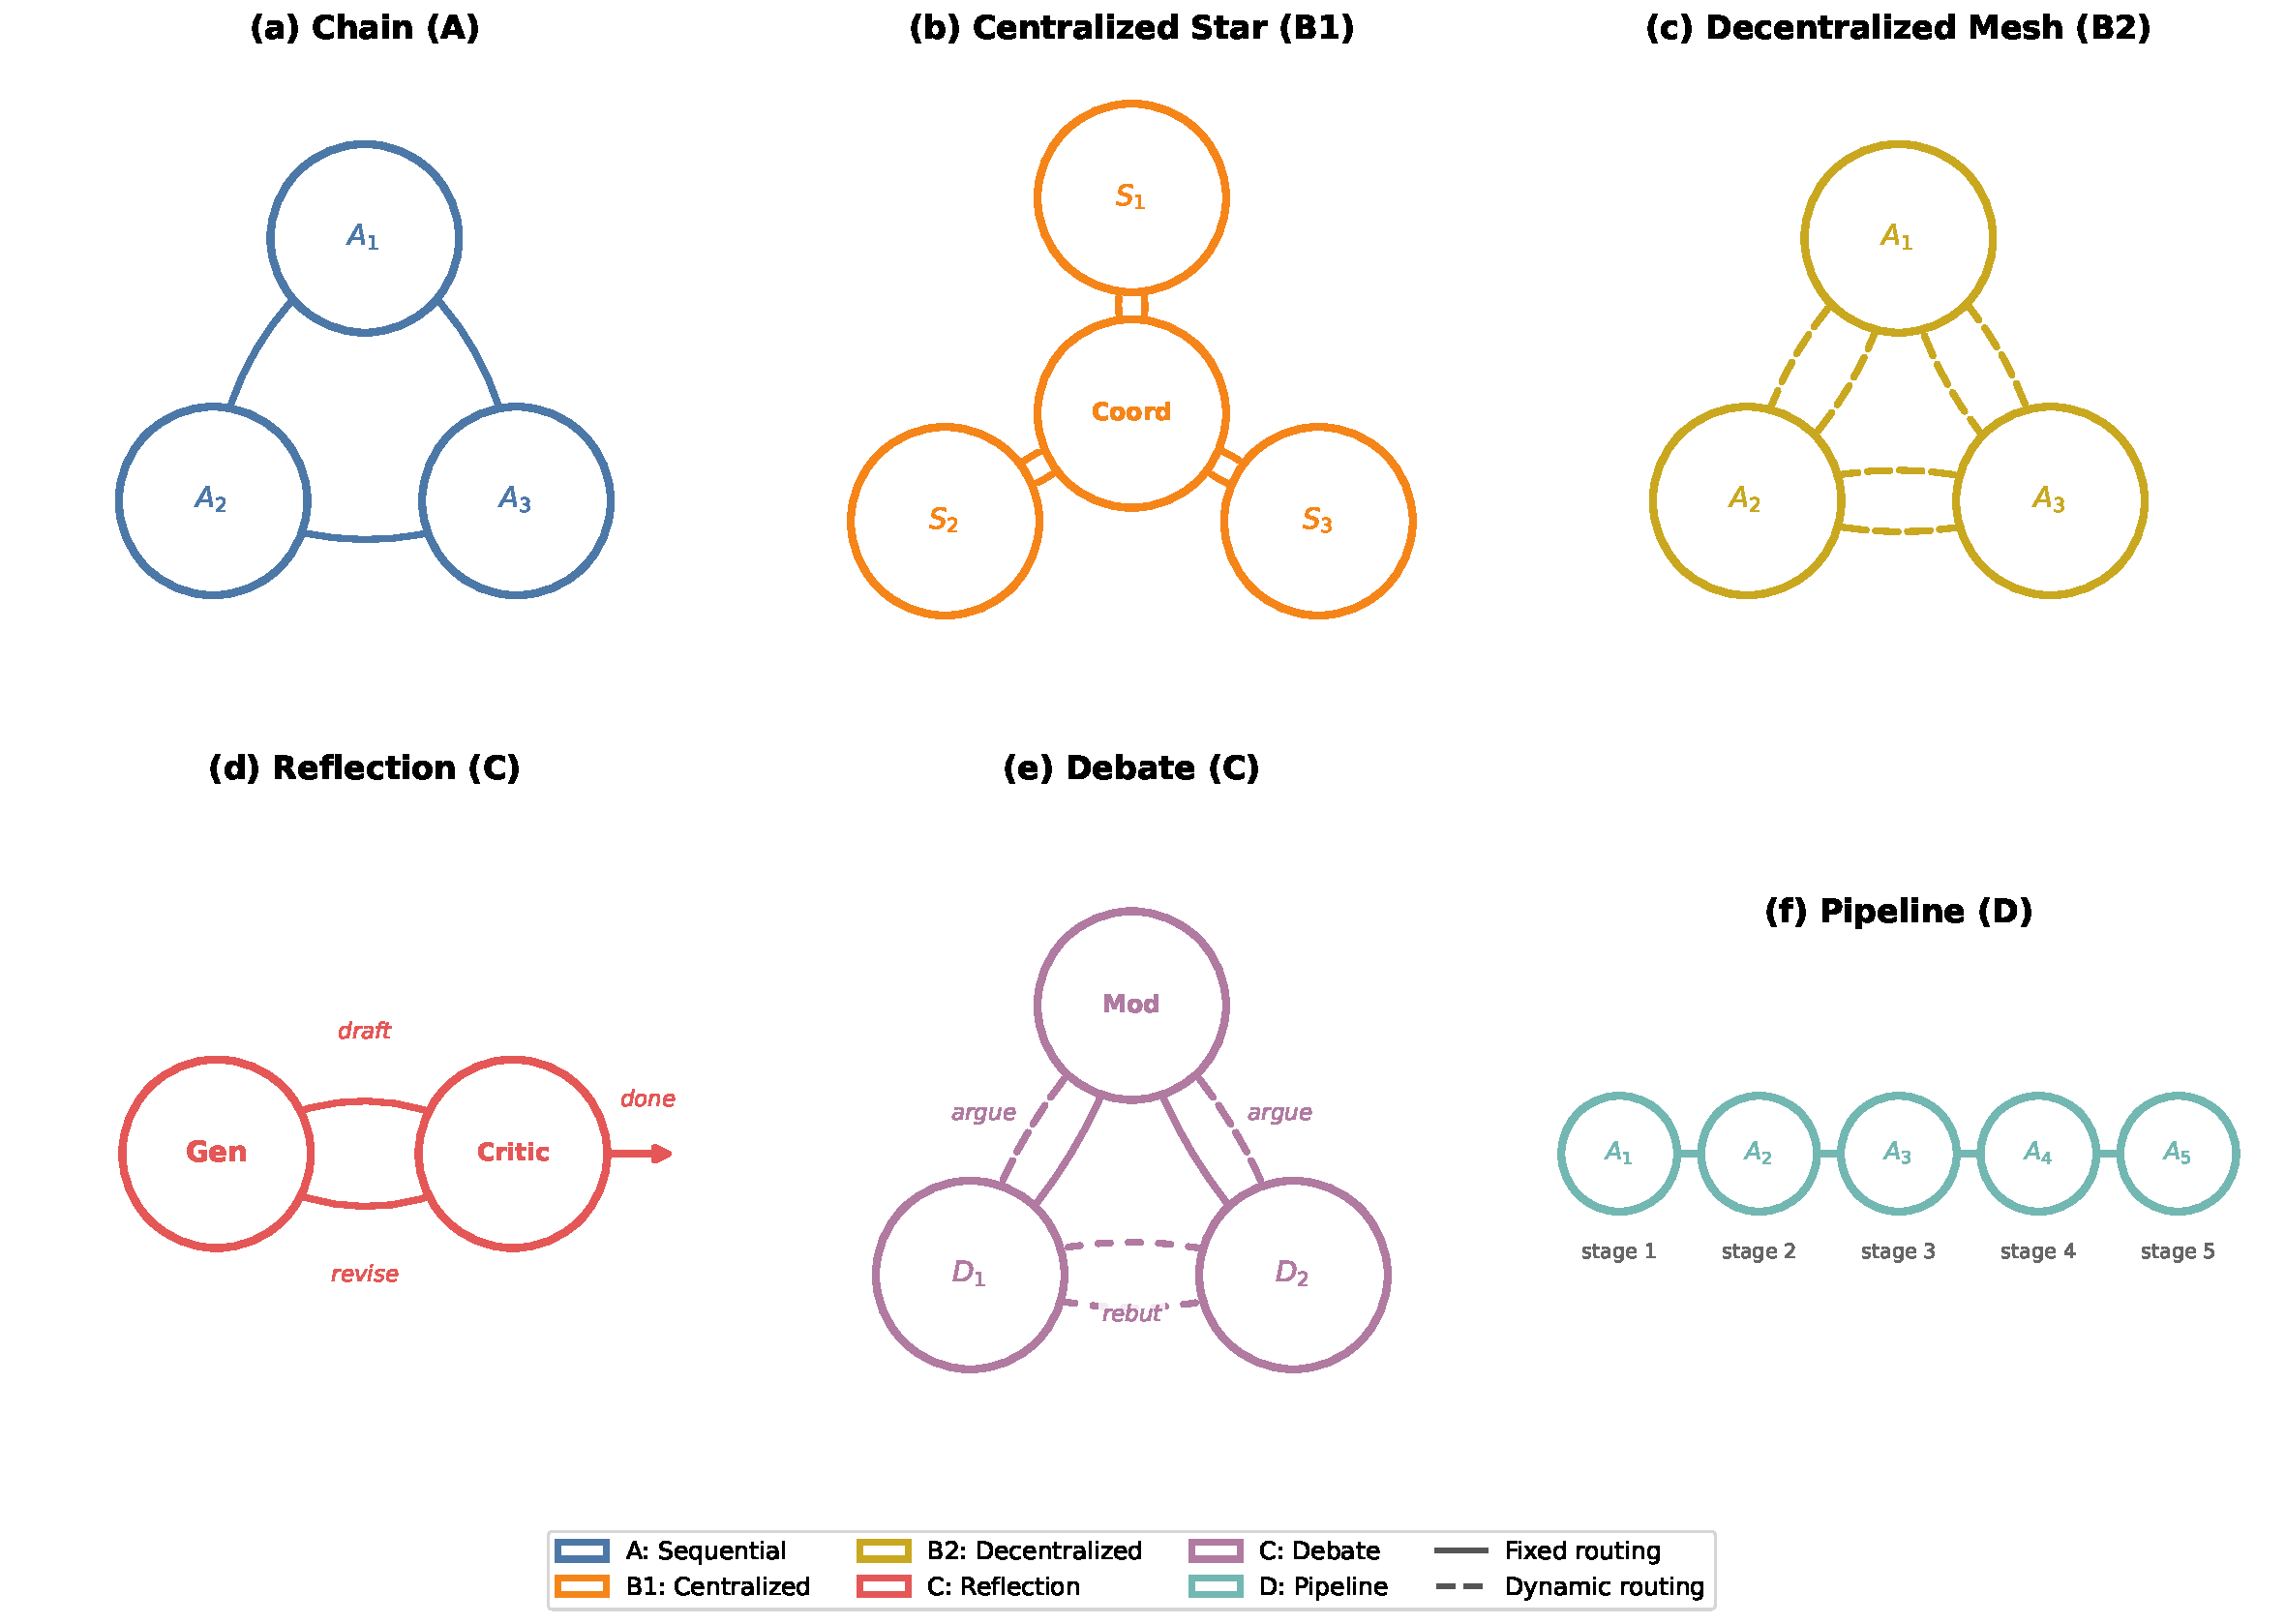
\includegraphics[width=\linewidth]{fig1_taxonomy.pdf}
    \caption{13가지 조정 패턴의 5개 범주 분류 체계. 체인(A), 스타(B1), 메시(B2), 피드백(C), 복합(D) 토폴로지.}
    \label{fig:taxonomy}
\end{figure}

\textbf{고정 순차 (범주 A) --- 체인 토폴로지.} 라운드 로빈 패턴은 고정 순서로 에이전트를 순환: $\text{Agent}_1 \to \text{Agent}_2 \to \cdots \to \text{Agent}_n \to \text{Agent}_1$. 각 에이전트는 전체 대화 이력을 보지만 라우팅에 영향을 미칠 수 없다. 이는 Masterman et al.의 체인/워터폴 토폴로지에 해당하며, MetaGPT (Hong et al., 2024)의 SOP 기반 순차 핸드오프와 동일한 구조다. 패턴: RR-2, RR-3, RR-4.

\textbf{중앙 집중형 라우팅 (범주 B1) --- 스타 토폴로지.} 전용 조정자 에이전트(Selector)가 대화 상태를 분석하여 다음 호출할 전문가를 \textbf{중앙에서 결정}한다. 이는 Masterman et al.의 스타/허브-앤-스포크 토폴로지에 해당하며, AutoGen의 SelectorGroupChat이 대표적 구현이다. 각 라우팅 결정마다 LLM 호출 오버헤드가 발생하나, 조정자가 전역 상태를 파악하여 최적 전문가를 선택할 수 있다. 패턴: Sel-3, Sel-4.

\textbf{탈중앙 핸드오프 (범주 B2) --- 메시 토폴로지.} 중앙 조정자 없이 각 에이전트가 \textbf{자율적으로 다음 에이전트에게 핸드오프}한다. 이는 Masterman et al.의 메시/스웜 토폴로지에 해당하며, OpenAI Swarm (2024)의 경량 핸드오프 루틴이 대표적이다. 에이전트 간 직접적 P2P 통신으로 조정 병목이 없으나, 턴 폭증(turn explosion)의 위험이 있다. 패턴: Swm-3, Swm-4.

\begin{quote}
\textbf{범주 B의 분리 근거.} 기존 연구에서 Selector와 Swarm을 ``동적 라우팅''으로 통합하였으나, 본 실험 결과 양자의 행동이 근본적으로 상이함을 확인하였다: Selector는 소수의 긴 모놀로그(2,100 tok/turn)를, Swarm은 다수의 짧은 핸드오프(330 tok/turn)를 생성한다. 스케일링 방향도 정반대로, Selector는 아선형($\text{sel4}/\text{sel3}=1.48\times$)이나 Swarm은 초선형($\text{swm4}/\text{swm3}=3.17\times$)이다. Tran et al. (2025)의 5-차원 협업 프레임워크에서도 \emph{구조(Structure)} 차원에서 ``중앙 집중형(centralized) vs.\ 분산형(distributed)''을 명시적으로 분리하여, 이 구분의 학술적 정당성을 지지한다.
\end{quote}

\textbf{구조화 피드백 (범주 C).} 에이전트가 명시적 피드백 루프를 통해 출력을 반복 정제한다. 반성(reflection) 패턴 (NeurIPS 2024)은 생성자와 비평가를 쌍으로 구성하고, 토론(debate) 패턴 (Du et al., ICML 2024)은 에이전트가 중재자와 함께 논거를 교환한다. 이 토폴로지는 수렴할 수 있으나 진동의 위험도 있다. 패턴: Refl-2, Refl-3, Deb-3, Deb-4.

\textbf{복합/중첩 (범주 D).} 다수의 단계 또는 계층이 파이프라인 또는 혼합 에이전트(MoA) 아키텍처로 구성된다. 파이프라인 패턴은 체인 토폴로지의 확장(체인의 체인)으로 순차 정제 단계를 통해 과제를 처리하고, MoA (ICLR 2025)는 다수의 병렬 응답을 생성 후 집약한다. 패턴: Pipe, MoA.

선행 프레임워크는 이 패턴의 부분 집합을 구현했다: AutoGen (Wu et al., 2023)은 라운드 로빈, 선택자, 스웜 패턴을 지원하고; DyTopo (Lu et al., 2026)는 라운드마다 희소 그래프를 재구성하는 동적 토폴로지 전환을 지원하며; MoA (ICLR 2025)는 계층적 집약 패턴을 도입한다. Wang et al. (2025)은 소세계 네트워크 이론을 멀티 에이전트 토론에 적용하여 원칙적 토폴로지 설계가 합의 궤적을 안정화하면서 토큰 효율성을 유지함을 보였다. MegaAgent (ACL 2025)는 대규모에서 에이전트 간 대화 토큰이 총 비용을 지배함을 보여, 토폴로지 인식 통신 효율의 필요성을 제기한다. G-Designer (Zhang et al., ICML 2025)는 변분 그래프 오토인코더로 과제 특화 통신 토폴로지를 동적 생성하여, HumanEval에서 최대 95.33\% 토큰 절감을 달성했다. AgentDropout (Wang et al., ACL 2025)은 통신 그래프 인접 행렬을 최적화하여 중복 에이전트를 동적 제거하며, 21.6\% 프롬프트 토큰 절감과 1.14점 성능 향상을 동시 달성한다. 본 연구는 이를 보완하여 \emph{종료 역학}에 집중한다---어떤 토폴로지를 선택할 것인가가 아니라, \textbf{선택된 토폴로지 내에서 팀이 언제 멈춰야 하는가}를 연구한다.

\subsection{LLM 시스템의 종료 기준}

\textbf{단일 에이전트 종료.} REFRAIN (Sun et al., 2025)은 연쇄 사고(Chain-of-Thought) 추론에서의 ``과잉 사고(overthinking)''를 이중 단계 정지 판별기와 슬라이딩 윈도우 UCB 다중 슬롯머신 제어기로 해결하여, 정확도를 유지하면서 토큰 사용량을 20--55\% 절감한다. 자기 일관성 샘플링 (Wang et al., 2023)은 다수의 추론 경로가 합의할 때 암묵적으로 수렴 감지를 사용한다.

\textbf{멀티 에이전트 종료.} Hu et al. (NeurIPS 2025)은 멀티 에이전트 토론을 위한 적응적 안정성 감지를 제안하여, 베타-이항 분포에 대한 KS 통계량으로 심판 의견이 안정화되는 시점을 감지한다 (통상 2--7라운드). Ruan \& Wang (2025)은 점진적 쿼럼 감지를 통한 조기 종료가 가능한 형식적 합의 프로토콜 Aegean을 도입하여, 답변 품질을 2.5\% 이내로 유지하면서 1.2--20배 지연 시간 절감을 달성한다. Cemri et al. (2025)은 멀티 에이전트 시스템의 3대 실패 범주 중 하나로 종료를 식별하며, 무한 루프와 조기 종료 실패를 문서화한다. SupervisorAgent (Lin et al., 2025)는 LLM 없는 컨텍스트 필터를 통한 런타임 적응적 감독으로, GAIA 벤치마크에서 성공률 저하 없이 토큰 소비를 29.45\% 절감한다.

\textbf{갭(Gap).} 포괄적인 조정 토폴로지 집합에서 종료 역학이 어떻게 변하는지를 체계적으로 연구한 선행 연구는 없다. 기존 적응적 종료는 특정 설정을 대상으로 한다: Hu et al. (2025)은 토론 패턴, Aegean은 병렬 합의, REFRAIN은 단일 에이전트 CoT. G-Designer는 토폴로지 선택을 최적화하지만 선택된 토폴로지 내에서 언제 멈출지는 연구하지 않는다. AgentDropout은 \emph{어떤 에이전트가} 참여할지를 최적화하지만 \emph{언제} 종료할지는 다루지 않는다. 본 연구는 5개 범주의 13개 패턴을 연구하고, 토폴로지 인식 적응적 종료를 제안하며, 팀이 언제 멈춰야 하는지에 대한 실증적 가이드라인을 제공함으로써 이 갭을 메운다.

\subsection{멀티 에이전트 출력의 품질 평가}

품질 지표로 G-Eval (Liu et al., 2023)을 채택하며, 평가자 LLM으로 Claude Sonnet 4.5를 사용한다. G-Eval은 인간 판단과 높은 상관이 입증된 구조화된 텍스트 품질 평가 프레임워크를 제공한다. 5개 과제 관련 차원으로 적응: 정확성(accuracy), 완전성(completeness), 일관성(coherence), 유용성(usefulness), 종합(overall), 각각 1--5 정수 척도. 오류 감지를 위해 MAST 범주와 정렬한 분류 체계를 사용한다: 환각, 사실 오류, 불완전성, 불일치, 무관성.

\begin{table}[H]
\centering
\caption{관련 연구 비교}
\label{tab:related-work}
{\small
\begin{tabular}{lcccc}
\toprule
\textbf{연구} & \textbf{패턴 수} & \textbf{토폴로지 범주} & \textbf{적응적 종료} & \textbf{수렴 감지} \\
\midrule
MAST (Cemri et al., 2025) & 2 & 토론, 투표 & 없음 & 궤적 수준 \\
REFRAIN (2025) & 1 & CoT (단일) & 있음 (판별기+UCB) & 해당 없음 \\
Hu et al. (NeurIPS 2025) & 1 & 토론 & 있음 (KS-검정) & 분포 수준 \\
Aegean (Ruan \& Wang, 2025) & 해당 없음 & 병렬 합의 & 있음 (쿼럼) & 쿼럼 수준 \\
Cemri et al. (2025) & ${\sim}5$ & 혼합 & 없음 & 사후 분석 \\
G-Designer (ICML 2025) & 동적 & GNN 생성 & 없음 (과제별 고정) & 해당 없음 \\
Scaling Agent Systems (2025) & 5 & 4개 조정 유형 & 없음 & 해당 없음 \\
Wang et al. (2025) & 1 & 토론 (소규모 세계) & 없음 & 의미 엔트로피 \\
AgentDropout (ACL 2025) & 가변 & 통신 그래프 & 없음 (에이전트 제거) & 해당 없음 \\
SupervisorAgent (2025) & 1+ & 런타임 감독 & 있음 (LLM-프리 필터) & 컨텍스트 수준 \\
\midrule
\textbf{본 연구} & \textbf{14} & \textbf{6개 범주} & \textbf{있음 (토폴로지 인식)} & \textbf{주장 수준 KS-검정} \\
 & & & & \textbf{+ 비용 예측 + 난이도 상호작용} \\
\bottomrule
\end{tabular}
}
\end{table}

%% ========================================================
\section{방법론}
%% ========================================================

\subsection{패턴 분류 체계}

고전적 MAS 토폴로지 이론 (Masterman et al., 2025)의 3대 정규 토폴로지(체인, 스타, 메시)에 피드백 루프와 복합 아키텍처를 추가하여, \textbf{5개 범주}로 조직된 13가지 조정 패턴을 연구한다 (그림~\ref{fig:taxonomy}). 각 패턴은 에이전트 수 $n$으로 매개변수화되며, 공통 종료 어휘를 공유한다 (정상 종료를 위한 TERMINATE 키워드, 안전 상한으로 \texttt{max\_messages}=25).

\begin{table}[H]
\centering
\caption{패턴 구성}
\label{tab:patterns}
{\small
\begin{tabular}{llllcll}
\toprule
\textbf{패턴} & \textbf{범주} & \textbf{토폴로지} & \textbf{에이전트} & \textbf{역할} & \textbf{라우팅} & \textbf{종료} \\
\midrule
Solo & S & 단일 & 1 & 범용 어시스턴트 & N/A & 키워드 또는 최대 \\
RR-2 & A & 체인 & 2 & 작성자, 연구자 & 고정 라운드 로빈 & 키워드 또는 최대 \\
RR-3 & A & 체인 & 3 & 작성자, 연구자, 검토자 & 고정 라운드 로빈 & 키워드 또는 최대 \\
RR-4 & A & 체인 & 4 & 작성자, 연구자, 검토자, 편집자 & 고정 라운드 로빈 & 키워드 또는 최대 \\
Sel-3 & B1 & 스타 & 3+1 & 전문가 3 + 선택자 & 중앙 LLM 라우팅 & 키워드 또는 최대 \\
Sel-4 & B1 & 스타 & 4+1 & 전문가 4 + 선택자 & 중앙 LLM 라우팅 & 키워드 또는 최대 \\
Swm-3 & B2 & 메시 & 3 & 핸드오프 전문가 3 & 자율 P2P 핸드오프 & 키워드 또는 최대 \\
Swm-4 & B2 & 메시 & 4 & 핸드오프 전문가 4 & 자율 P2P 핸드오프 & 키워드 또는 최대 \\
Refl-2 & C & 피드백 & 2 & 생성자, 비평가 & 피드백 고정 & 키워드 또는 최대 \\
Refl-3 & C & 피드백 & 3 & 생성자, 비평가, 정제자 & 피드백 고정 & 키워드 또는 최대 \\
Deb-3 & C & 피드백 & 3+1 & 토론자 3 + 중재자 & 중재 & 키워드 또는 최대 \\
Deb-4 & C & 피드백 & 4+1 & 토론자 4 + 중재자 & 중재 & 키워드 또는 최대 \\
Pipe & D & 체인의 체인 & 2+ & 단계별 팀 & 순차 단계 & 단계별 키워드 \\
MoA & D & 팬아웃/집약 & 3+ & 병렬 + 집약자 & 팬아웃/집약 & 집약자 결정 \\
\bottomrule
\end{tabular}
}
\end{table}

\subsection{과제 모음}

25개 과제를 \textbf{2차원}으로 분류한다: \emph{인지 유형} (4개)과 \emph{주제 도메인} (9개). 이 이중 분류는 ``어떤 도메인에 어떤 토폴로지가 적합한가''를 분석할 수 있게 한다 (MultiAgentBench, ACL 2025; LegalAgentBench, ACL 2025 참조). 도메인 다양성을 극대화하여 도메인별 토폴로지 적합성 분석을 가능하게 한다.

\textbf{인지 유형 (4개):}
\begin{itemize}
    \item \textbf{사실형} (7개): 지식 검색 및 종합이 필요한 질문
    \item \textbf{분석형} (9개): 구조화된 추론과 비교 분석이 필요한 문제
    \item \textbf{창의형} (6개): 창의성, 대안 사고, 설계가 필요한 개방형 과제
    \item \textbf{기술형} (3개): 전문 기술 지식과 구현이 필요한 도메인 특화 과제
\end{itemize}

\textbf{주제 도메인 (9개):}
\begin{itemize}
    \item \textbf{과학} (3개): 열역학, 광합성, 암흑물질 검출
    \item \textbf{CS} (3개): 네트워킹, LRU 캐시 구현, 아키텍처 비교
    \item \textbf{역사} (3개): 1차 대전 원인, 제국 비교, 대안 역사
    \item \textbf{철학} (3개): 칸트 vs 밀, 트롤리 문제, 정체성 사고실험
    \item \textbf{법/정치} (3개): 삼권분립, AI 저작권, 자율주행 정책
    \item \textbf{게임} (3개): 게임 설계 원리, 매치메이킹, 교육 게임
    \item \textbf{공학} (3개): 구조 하중, 수처리장, 3D 프린팅 건설
    \item \textbf{경영} (3개): AI 교육 스타트업, VC vs 부트스트래핑, EV 시장 진출
    \item \textbf{의학} (1개): mRNA vs 단백질 백신
\end{itemize}

\begin{table}[H]
\centering
\caption{과제 분포 (인지유형 $\times$ 도메인)}
\label{tab:task-distribution}
\begin{tabular}{lccccc}
\toprule
\textbf{도메인} & \textbf{사실} & \textbf{분석} & \textbf{창의} & \textbf{기술} & \textbf{합계} \\
\midrule
과학 & 1 & 1 & 1 & 0 & 3 \\
CS & 1 & 1 & 0 & 1 & 3 \\
역사 & 1 & 1 & 1 & 0 & 3 \\
철학 & 1 & 1 & 1 & 0 & 3 \\
법/정치 & 1 & 1 & 1 & 0 & 3 \\
게임 & 1 & 0 & 1 & 1 & 3 \\
공학 & 1 & 1 & 0 & 1 & 3 \\
경영 & 0 & 2 & 1 & 0 & 3 \\
의학 & 0 & 1 & 0 & 0 & 1 \\
\midrule
\textbf{합계} & \textbf{7} & \textbf{9} & \textbf{6} & \textbf{3} & \textbf{25} \\
\bottomrule
\end{tabular}
\end{table}

v1 실험에서는 각 과제를 패턴당 3회 반복 실행하여 780회 실행 ($13\text{패턴} \times 20\text{과제} \times 3\text{반복}$)을 수행했다. v2 실험에서는 대표 패턴 8개에 대해 25개 과제를 각 1회 실행하여 200회 실행 ($8\text{패턴} \times 25\text{과제}$)을 수행한다.

전체 과제 목록과 프롬프트 원문은 부록 A의 표 A1에 수록한다. 각 프롬프트는 자기 완결적이며, 사실형 과제는 평균 25단어, 창의/기술형 과제는 평균 45단어이다. 본 메인 과제 모음은 중$\sim$고 난이도이며, 실험 07에서 명시적 쉬움/보통/어려움 등급을 도입한다.

\textbf{설계 근거: 개방형 과제.} 검증 가능한 벤치마크(HumanEval, MATH, MMLU 등)가 아닌 개방형 생성 과제를 \textbf{의도적으로} 선택했다. 종료 역학 연구에는 \textbf{턴에 걸쳐 품질이 연속적으로 변화}하는 과제가 필요하기 때문이다. 검증 가능한 벤치마크는 이진 결과(통과/실패)를 생성하여 턴별 품질 궤적, 수렴 패턴, 한계 효용 분석이 의존하는 점진적 품질 포화를 드러낼 수 없다. 개방형 과제는 최적 종료 시점 식별, 종료 후회 측정, 토폴로지 간 수렴 속도 비교에 필요한 풍부한 품질 곡선을 생성한다. 이 설계 선택은 관련 멀티 에이전트 평가 연구와 일치한다: MAST (Cemri et al., 2025)는 궤적 수준 품질 연구에, Hu et al. (2025)는 수렴 연구에 개방형 과제를 사용한다. 코드 생성이나 수학적 추론에서의 종료 역학은 다를 수 있으며 (5.3절), 이러한 과제로의 확장은 중요한 향후 방향이다.

\subsubsection{에이전트 시스템 프롬프트}

각 에이전트는 전문성과 행동 기대치를 정의하는 역할별 시스템 프롬프트를 받는다. 모든 프롬프트는 공통 구조를 공유한다: (1) 역할 정의, (2) 응답 가이드라인, (3) 종료 지시 (``과제가 완료되면 TERMINATE라고 말하세요'').

\textbf{범주 A (라운드 로빈):} 에이전트에 상호 보완적 역할---Writer(초안 생성), Researcher(사실 보강), Reviewer(완전성 평가), Editor(문체 정제)---을 부여한다. 각 에이전트는 처음부터 다시 쓰지 않고 선행 기여에 기반하도록 지시받는다.

\textbf{범주 B1 (셀렉터):} 셀렉터 에이전트는 라우팅 프롬프트를 받는다: ``대화를 분석하고 다음 턴에 가장 적합한 전문가를 선택하세요.'' 전문가 에이전트는 범주 A와 동일한 역할 프롬프트를 받는다.

\textbf{범주 B2 (스웜):} 각 에이전트는 핸드오프 도구(\texttt{transfer\_to\_<agent>})를 받으며, ``당신의 부분을 완료한 후 다음 단계에 적합한 에이전트에게 넘기세요. 과제가 완전히 해결되면 TERMINATE라고 말하세요''라는 지시를 받는다.

\textbf{범주 C (피드백):} 반성 패턴은 Generator(``포괄적 응답 생성'')와 Critic(``정확성, 완전성, 일관성 평가; 구체적 피드백 제공 또는 만족스러우면 APPROVED'')을 사용한다. 토론 패턴은 Debater(``주제에 대한 가장 강력한 논거 제시'')와 Moderator(``논거 종합 후 합의 또는 입장이 명확해지면 VERDICT 발행'')를 사용한다.

\textbf{범주 D (복합):} 파이프라인은 순차 전문가를, MoA는 병렬 생성자와 Aggregator(``모든 응답의 최선 요소를 통합 답변으로 결합'')를 사용한다.

14개 패턴의 전체 시스템 프롬프트는 보충 코드 저장소에서 제공한다.

\subsection{실험 프레임워크}

모든 실험은 통합 멀티 에이전트 프레임워크(AutoGen)와 Claude Haiku 4.5를 기반 모델로 사용한다. 교차 모델 일반화를 평가하기 위해 실험 01을 GPT-4o-mini로 5개 대표 패턴에서 복제하고(4.6절), 4개 제공자 계열의 5개 독립 모델로 품질 점수를 교차 검증한다(4.2.1절). 다중 가설 검정에 대해 Benjamini-Hochberg 위발견율(FDR) 보정을 $q < 0.05$에서 적용하며, 보고된 모든 유의 효과는 보정을 통과한다.

\textbf{실행별 캡처 지표:}
\begin{itemize}
    \item \emph{지속 시간}: \texttt{team.run()} 시작부터 완료까지의 벽시계 시간
    \item \emph{턴 수}: 대화의 총 메시지 수
    \item \emph{에이전트 턴 수}: 비시스템 에이전트의 메시지 수
    \item \emph{토큰 사용량}: LLM 호출별 프롬프트 토큰(입력)과 완성 토큰(출력)
    \item \emph{종료 사유}: 팀 종료 방식 (키워드, \texttt{max\_messages}, 오류)
    \item \emph{품질 점수}: G-Eval 평가 (실험 02만)
    \item \emph{수렴 지점}: KS-검정 안정성 (실험 03만)
\end{itemize}

\subsection{7개 실험}

\textbf{실험 01: 패턴 효율성} (780회). 전체 과제 모음에서 13개 패턴의 지속 시간, 턴 수, 에이전트 턴, 토큰 사용량을 비교한다. Kruskal--Wallis 검정으로 토폴로지 범주가 효율의 유의한 예측 변수인지 검증한다.

\textbf{실험 02: 종료 품질} (100회). 5개 대표 패턴(범주당 하나)에 대해 20개 과제에서 각 에이전트 턴에 G-Eval 스코어링을 적용하여 품질 궤적을 구축한다 (100회 실행, 276개 턴별 품질 점수). 종료 후회(실제와 최적 종료 시점의 차이)를 식별한다.

\textbf{실험 03: 수렴 감지} (분석만). 실험 01의 메시지 데이터로 KS-검정 수렴 지표를 산출하여, 범주 간 수렴 속도를 비교한다. 피드백 패턴이 순차 패턴보다 빠르게 수렴하는지 검증한다.

\textbf{실험 04: 오류 귀인} (분석만). 실험 01과 02의 오류를 8개 유형으로 분류하고, 토폴로지 특성과의 오류 분포 상관을 분석한다. 패턴별 오류 시그니처를 검증한다.

\textbf{실험 05: 적응적 종료} (800회). 적응적 $\Delta U$ 기반 종료와 키워드 베이스라인을 비교하는 통제 실험. 8개 대표 패턴 전체에서 25개 과제를 3개 $\lambda$값(0.0, 0.1, 0.5)으로 실행하여 200회 베이스라인 + 600회 적응적 = 800회 실행. $\Delta U(t) = \Delta Q(t) - \lambda \cdot \Delta C(t) \to 0$이 실용적 종료 신호로 기능하는지 평가한다.

\textbf{실험 06: 토폴로지 특성 기반 비용 예측} (분석만). 실험 01 데이터(718회)로 4개 회귀 모델(선형, Ridge, Lasso, Random Forest)을 학습하여, 사전 실행 토폴로지 특성(패턴 범주, 에이전트 수, 최대 메시지 수, 과제 범주, 상호작용 항 \texttt{agent\_count $\times$ max\_messages})으로 런타임 비용(토큰, 턴 수, 지속 시간)을 예측한다. 5-fold 교차 검증과 실험 05 베이스라인 데이터(200회)에 대한 홀드아웃 예측으로 평가한다.

\textbf{실험 07: 과제 난이도 상호작용} (225회). 5개 대표 패턴(solo, swm3, sel3, refl2, debate3---범주당 하나)과 15개 난이도 등급 과제(5개 도메인 $\times$ 3개 난이도: 쉬움, 보통, 어려움)를 3회 반복으로 교차한다. Kruskal--Wallis 검정으로 주효과 및 상호작용을 검증하고, G-Eval 채점으로 난이도 인식 추천 매트릭스를 도출한다.
%% main_kr_part2.tex — \input from main Korean file
%% Starts at \section{결과}, ends with \end{document}

\section{결과}
\label{sec:results}

7개 상호 연결 실험의 결과를 각 연구 질문에 대응하여 제시한다. 모든 실험은 커스텀 AutoGen ChatCompletionClient를 통해 Claude Haiku 4.5를 기반 모델로 사용하여, 13개 조정 패턴과 단일 에이전트 베이스라인에서 일관된 LLM 행동을 보장한다.

\subsection{실험 01: 패턴 효율성 (RQ1)}

\textbf{설정.} 780회 실행 (13패턴 $\times$ 20과제 $\times$ 3반복)과 25회 단일 에이전트 베이스라인 실행을 수행하여 실행별 지속 시간, LLM 호출 수, 토큰 소비를 측정했다. 인프라 오류 (28K 문자 초과 프롬프트 절단) 발생 실행은 분석에서 제외했다.

\subsubsection{단일 에이전트 베이스라인 (카테고리 S)}

멀티 에이전트 오버헤드의 하한선을 설정하기 위해, 25개 태스크에 대해 단일 범용 에이전트를 실행하였다 (max\_messages=5, TERMINATE 키워드 종료).

% [표 tab:solo-baseline → 부록 이동]

\paragraph{발견 1: 멀티 에이전트 조정은 단일 에이전트 대비 3.3--6.1배의 토큰 오버헤드를 발생시킨다.}
Solo 베이스라인은 25개 태스크를 평균 1,287 토큰, 100\% 키워드 종료율로 완료하여 하한선을 설정한다. 가장 저렴한 멀티 에이전트 패턴(swm3, 3 에이전트)은 3.26배 더 많은 토큰을 사용하며, rr2(2 에이전트)는 3.70배이다. 이 오버헤드는 에이전트 간 통신, 컨텍스트 축적, 턴 프로토콜의 \emph{조정 비용}을 정량화한다. 다만 이 오버헤드는 품질 향상과 비교하여 평가해야 한다: 실험 02의 멀티 에이전트 품질 분석에서 멀티 에이전트 패턴이 더 높은 G-Eval 점수를 달성함을 보여준다.

\subsubsection{범주 A: 고정 순차 패턴}

표~\ref{tab:cat-a-efficiency} (부록)은 범주 A (고정 순차)의 결과를 제시하며, 에이전트 수가 고정 라운드 로빈 토폴로지의 효율에 미치는 영향을 보여준다.

% [표 tab:cat-a-efficiency → 부록 이동]

% [표 tab:cat-a-three → 부록 이동]

참고: rr4의 71.7\% 오류율은 인프라 버그로 인한 과대평가다 (4.4절). 성공한 rr4 17회 실행은 주로 사실형 과제(15/17)로, 지표가 짧은 과제 쪽으로 편향되었다. 범주 B/C/D는 수정된 인프라 코드를 사용한다.

\paragraph{발견 2: 입력 토큰 증가에 의한 준선형 비용 확장.}
에이전트 추가는 지속 시간을 약 2배 (rr3/rr2=1.84배), 총 토큰을 약 2배 (2.13배) 증가시키며, 이는 준선형 확장과 일치한다. 사실형 과제만의 비교 (표~\ref{tab:cat-a-three}, 부록)는 흥미로운 추세를 보여준다: LLM 호출당 출력 토큰이 팀 규모에 따라 \emph{증가}한다 (rr2=930, rr3=1,189, rr4=1,544; rr2에서 rr4로 1.66배). 이는 에이전트가 더 많은 선행 기여에 노출될수록 더 풍부한 응답을 생성함을 시사하며---\textbf{협력적 증폭(collaborative amplification)} 현상과 일치한다. 비용 주요 동인은 \emph{입력 토큰 축적}이다: 입력 토큰은 2.59배 증가 (LLM 호출의 1.75배 대비)하여, 라운드 로빈의 각 에이전트가 전체 대화 이력을 보는 것을 확인한다.

\paragraph{발견 3: 입력 토큰 초선형 증가.}
입력 토큰은 2.59배 증가 (LLM 호출의 1.75배 대비)하여, 초선형 컨텍스트 축적을 보인다. 예상 이론적 증가는 $O(n \cdot k \cdot L)$이며, $n$=에이전트 수, $k$=라운드, $L$=평균 응답 길이이다.

\paragraph{발견 4: 에이전트 수에 따른 오류율 초선형 증가.}
오류율이 극적으로 증가한다: rr2=8.3\%, rr3=23.3\%, rr4=71.7\%. 과제 범주별 오류 분포는 단조적으로 확대된다: rr2 오류는 기술형 과제에만 집중 (5/5 오류), rr3는 기술형(8/14), 창의형(3/14), 분석형(3/14)으로 확산, rr4는 비사실형 범주 전반에서 거의 완전 실패에 도달한다. 사실형 과제만이 세 패턴 모두에서 0\% 오류율을 유지한다.

\paragraph{발견 5: 과제 범주 효과.}
과제 범주에 따른 유의한 변동을 관찰한다 (표~\ref{tab:task-category-effect}, 부록). 창의형 과제는 가장 긴 시간(93.3초 평균)을 요구하고, 사실형 과제가 가장 효율적이다 (66.5초, 6,183 토큰). 기술형 과제는 최고 토큰 밀도(9,100 평균)와 최고 오류율(42.1\%)을 보이며, 이는 컨텍스트 오버플로를 유발하는 긴 코드 생성 응답에 기인한다.

% [표 tab:task-category-effect → 부록 이동]

\subsubsection{범주 B1 (중앙 집중 라우팅) 및 B2 (분산 핸드오프) 비교}

표~\ref{tab:cat-b} (부록)는 범주 B1 (Star: SelectorGroupChat 기반, 중앙 LLM 라우터가 다음 발언자 선택)과 B2 (Mesh: Swarm 기반, 에이전트가 Handoff 도구 호출로 자율 위임)의 결과를 비교한다. 240회 실행 모두 0\% 오류율로 성공하여, 인프라 수정이 범주 A의 프롬프트 절단 문제를 해결했음을 확인한다.

% [표 tab:cat-b → 부록 이동]

\paragraph{발견 6: B1 (Star)과 B2 (Mesh)가 근본적으로 다른 턴 수준 행동을 생성한다.}
B1 선택자 패턴은 소수의 턴(3.5--4.1)에서 긴 독백(턴당 2,114--2,616 출력 토큰)을 생성하는 반면, B2 스웜 패턴은 다수의 턴(10.2--25.0)에서 짧고 집중된 핸드오프(턴당 330--337 출력 토큰)를 생성한다. 스웜 접근법이 3에이전트에서 유의하게 더 효율적이다: 선택자 대비 35\% 빠르고 47\% 저렴하다.

\paragraph{발견 7: 중앙 집중(B1) vs 분산(B2) 라우팅이 반대의 확장 행동을 결정한다.}
B1 선택자 확장은 차선형: sel4/sel3 = 1.48배 총 토큰. B2 스웜 확장은 초선형: swm4/swm3 = 3.17배 총 토큰. 3에이전트에서 swm3가 sel3보다 47\% 저렴하나, 4에이전트에서 swm4가 sel4보다 15\% 비싸다. 이 교차점은 실용적 의미를 가진다: 소규모 팀($n \leq 3$)에는 스웜 라우팅을, 대규모 팀에는 선택자 라우팅을 선호해야 한다.

\paragraph{발견 8: Swm-3가 최고의 전체 토큰 효율을 달성한다.}
놀랍게도 swm3 (3에이전트 스웜)가 rr2 (2에이전트 라운드 로빈)보다도 낮은 총 토큰 비용을 달성한다 (4,196 vs 4,759). 50\% 더 많은 에이전트로 12\% 비용 절감은, 지능적 라우팅이 추가 에이전트의 오버헤드를 상쇄하고도 남음을 보여준다.

% [표 tab:cross-ab → 부록 이동]

비교 결과 라우팅 전략이 에이전트 수보다 효율에 더 큰 영향을 미침을 알 수 있다. swm3는 동일 에이전트 수에도 rr3보다 59\% 적은 토큰을 사용하고, sel3는 조정자 에이전트를 추가했음에도 rr3보다 22\% 적은 토큰을 사용한다.

\subsubsection{범주 C: 구조화 피드백 패턴}

표~\ref{tab:cat-c} (부록)은 범주 C (구조화 피드백)의 결과를 제시하며, 반성 기반 패턴(생성자-비평가 루프)과 토론 기반 패턴(중재자 포함 다자 논증)을 비교한다. 240회 전부 0\% 오류율로 성공했다.

% [표 tab:cat-c → 부록 이동]

\paragraph{발견 9: 반성과 토론이 반대의 확장 행동을 보인다.}
반성 확장은 초선형: refl3/refl2 = 2.31배 총 토큰. 토론 확장은 차선형: deb4/deb3 = 1.25배 총 토큰. 이 대조는 피드백의 \emph{존재} 여부보다 피드백 \emph{구조}가 확장 효율에 더 중요함을 밝힌다.

\paragraph{발견 10: Refl-2가 품질 보증과 함께 준베이스라인 효율을 달성한다.}
refl2 (60.2초, 5,237 토큰)는 전체 범주 최저가인 rr2 (52.4초, 4,759 토큰) 대비 15\% 느리고 10\% 비쌀 뿐이다. 그러면서도 refl2는 고정 순차 패턴에 없는 구조화된 비평-승인 루프를 포함한다.

\paragraph{발견 11: 동일 에이전트 수에서 반성은 빠르고 토론은 저렴하다.}
refl3과 deb3 (모두 3에이전트) 비교: refl3이 30\% 빠르지만 (120.2초 vs 156.6초) 30\% 더 많은 토큰을 생성한다 (12,095 vs 9,313).

\paragraph{발견 12: 토론이 팀 성장 시 에이전트별 출력을 제약한다.}
토론에서 에이전트 턴당 출력 토큰이 팀 규모에 따라 \emph{감소}한다 (deb3=1,691, deb4=1,448; 0.86배). 이는 범주 A에서 관찰된 턴당 출력 \emph{증가}의 협력적 증폭과 대조된다.

\subsubsection{범주 D: 복합 패턴}

표~\ref{tab:cat-d} (부록)은 범주 D (복합/중첩)의 결과를 제시한다. 120회 전부 0\% 오류율로 성공했다.

% [표 tab:cat-d → 부록 이동]

% [표 tab:cat-d-task → 부록 이동]

\paragraph{발견 13: MoA는 전체 패턴 중 가장 비싸다.}
MoA의 평균 총 토큰(22,333)은 13개 패턴 중 최고치이며, pipe 대비 61\%, 전체 최저 비용인 swm3 대비 5.3배에 달한다. 출력 토큰(17,458)이 입력 토큰(4,875)의 3.58배로, 전체 패턴 중 가장 극단적인 출력 편향을 보인다.

\paragraph{발견 14: 복합 패턴은 최고 출력 밀도를 보인다.}
에이전트 턴당 출력 토큰이 pipe=2,325, MoA=2,494로, 전체 13개 패턴 중 가장 높다. 복합 패턴이 에이전트 턴의 ``밀도''에서는 가장 효율적이나, 총 비용에서는 가장 비효율적이라는 역설적 결과를 낳는다.

\paragraph{발견 15: 과제 복잡도가 복합 패턴 비용을 기하급수적으로 증폭한다.}
MoA에서 기술형 과제(37,844 토큰)와 사실형 과제(15,064 토큰)의 비율은 2.51배로, 전체 패턴 중 가장 높은 과제 민감도를 보인다. 복합 패턴 배포 시 과제 복잡도 사전 평가가 비용 예측에 필수적임을 시사한다.

\begin{table}[H]
\centering
\caption{범주 간 효율 비교 (전체 14개 패턴)}
\label{tab:all-patterns}
{\footnotesize
\begin{tabular}{llcrrccc}
\toprule
패턴 & 범주 & 에이전트 & 시간(초) & 총 토큰 & $\pm$std & 95\% CI & vs solo \\
\midrule
solo  & S  & 1   & 18.7  & 1,287  & ---       & ---               & 1.00x \\
swm3  & B2 & 3   & 75.2  & 4,196  & $\pm$5,646 & [2,011; 6,672]   & 3.26x \\
rr2   & A  & 2   & 52.4  & 4,759  & ---       & ---               & 3.70x \\
refl2 & C  & 2   & 60.2  & 5,237  & $\pm$3,315 & [3,913; 6,649]   & 4.07x \\
sel3  & B1 & 3+1 & 115.2 & 7,851  & $\pm$5,243 & [6,338; 10,666]  & 6.10x \\
deb3  & C  & 3+1 & 156.6 & 9,313  & $\pm$2,501 & [7,625; 9,690]   & 7.23x \\
rr3   & A  & 3   & 96.6  & 10,121 & $\pm$10,148 & [8,143; 16,521] & 7.86x \\
sel4  & B1 & 4+1 & 161.9 & 11,595 & $\pm$6,428 & [8,610; 13,917]  & 9.01x \\
deb4  & C  & 4+1 & 180.9 & 11,637 & $\pm$2,978 & [10,875; 12,400] & 9.04x \\
refl3 & C  & 3   & 120.2 & 12,095 & $\pm$6,765 & [10,363; 13,828] & 9.40x \\
swm4  & B2 & 4   & 185.0 & 13,321 & $\pm$6,214 & [10,355; 15,486] & 10.35x \\
pipe  & D  & 5   & 129.6 & 13,856 & $\pm$5,828 & [10,780; 15,592] & 10.76x \\
moa   & D  & 4   & 103.0 & 22,333 & $\pm$10,599 & [19,618; 25,048] & 17.35x \\
\bottomrule
\end{tabular}
}

\smallskip
{\footnotesize 주: 표준편차 및 95\% 신뢰구간은 패턴당 $n=25$ 실행(v2 데이터셋)에서 산출. solo와 rr2는 개별 실행 데이터 부재. 전체 통계 분석은 부록~C 참조.}
\end{table}

표~\ref{tab:all-patterns}는 단일 에이전트 베이스라인을 포함한 14개 패턴을 총 토큰 비용으로 순위화하며, solo(1,287)에서 MoA(22,333)까지 17.4배 범위를 보여준다. 주요 관찰: (1) \emph{멀티 에이전트 오버헤드가 최소 3.3배}; (2) \emph{라우팅 전략이 에이전트 수를 지배}: swm3(3에이전트)가 rr2(2에이전트)보다 저렴; (3) \emph{피드백 패턴이 중간 대역 점유}; (4) \emph{복합 패턴이 고비용 대역 점유}; (5) \emph{출력 밀도 10배 차이}: swm3의 330 토큰/턴에서 MoA의 2,494 토큰/턴까지.

\subsubsection{범주 간 비교}

5개 토폴로지 범주에 대해 718회 성공 실행에 Kruskal-Wallis 검정을 적용하여 조정 토폴로지가 효율의 통계적으로 유의한 예측 변수인지 검증한다.

% [표 tab:kw-cross-cat → 부록 이동]

5개 지표 모두 중--대 효과 크기의 유의한 차이를 보인다. 턴 수가 가장 강한 범주 의존성($\eta^{2}=0.567$)을 보여, 토폴로지 범주가 턴 수 분산의 57\%를 설명함을 나타낸다.

% [표 tab:pairwise-mwu → 부록 이동]

% [표 tab:cat-token-summary → 부록 이동]

\paragraph{발견 16: B1/B2 분리가 기존 ``B $\approx$ C'' 등가를 해체한다.}
4범주 분석에서 ``B $\approx$ C'' ($p=0.112$)로 보였던 관계가, 5범주 분석에서는 \textbf{B2 $<$ C} ($p=0.028$, 유의)와 \textbf{B1 $\approx$ C} ($p=0.695$, 비유의)로 분해된다.

\paragraph{발견 17: 수정된 비용 위계---A $\approx$ B2 $<$ B1 $\approx$ C $\ll$ D.}
B1/B2 분리로 인해 비용 위계가 정교한 계층으로 재편된다. 특히 \textbf{A와 B2가 통계적으로 구분 불가능} ($p=0.857$)한 것은, 분산 핸드오프 토폴로지가 순차 체인과 동등한 비용 효율을 달성함을 의미한다.

% [표 tab:spearman-agents → 부록 이동]

\paragraph{발견 18: B1/B2의 에이전트 수 민감도 차이가 확장 비대칭을 설명한다.}
B2(분산)에서 에이전트 수와 턴 수의 상관이 B1(중앙 집중)보다 현저히 높다 ($\rho=0.704$ vs $\rho=0.377$). 분산 핸드오프에서 추가 에이전트가 핸드오프 체인의 조합적 증가를 유발하는 반면, 중앙 집중 라우터는 턴 수를 비교적 안정적으로 유지함을 반영한다.

\subsubsection{도메인 $\times$ 패턴 교차 분석}

\textbf{설정.} 8개 대표 패턴을 9개 지식 도메인에 걸친 25개 과제에서 평가한다 ($N=200$, 오류율 0\%).

% [표 tab:domain-pattern → 부록 이동]

% [표 tab:domain-cv → 부록 이동]

\paragraph{발견 19: debate3는 유일한 도메인 불변 패턴; swm3는 도메인 민감.}
8개 패턴 중 debate3가 가장 낮은 도메인 간 CV(0.14)를 보여, 도메인과 무관하게 비용이 일정하다. 반면 swm3는 최고 CV(0.67)로, 역사 과제에서 1,400 토큰이지만 경영에서 9,200 토큰이다.

\paragraph{발견 20: 반성 패턴이 논증적 도메인에서 탁월하나, 토론 패턴은 그렇지 않다.}
논증적 도메인(법/정치, 철학)에서 refl2가 가장 효율적인 패턴 중 하나이며, 철학에서는 최저 비용 패턴이다. 놀랍게도 debate3는 이 도메인에서 3--4위로, 논증이 자연스러운 영역에서 토론 구조가 우수할 것이라는 직관과 모순된다.

\paragraph{발견 21: 도메인 비용은 패턴 선택과 독립적으로 2배 변동.}
전 패턴 평균에서 가장 저렴한 도메인은 역사(7,063 토큰), 가장 비싼 도메인은 의학(13,288 토큰)으로 1.88배 차이가 난다.

%=========================================================================
\subsection{실험 02: 종료 품질 (RQ2)}
\label{sec:exp02}
%=========================================================================

\textbf{설정.} 범주당 대표 패턴에 대해 각 에이전트 턴마다 G-Eval 스코어링을 적용하여 품질 궤적을 구축한다. Claude Sonnet 4.5를 평가자로 사용하여 5차원 스코어링(정확성, 완전성, 일관성, 유용성, 종합)을 수행하며, 각 턴은 $Q(t) \in [1, 5]$ 품질 점수를 받는다.

\textbf{종료 후회}는 다음과 같이 정의한다:
\begin{equation}
R = t_{\text{actual}} - t_{\text{optimal}}
\end{equation}
여기서 $t_{\text{optimal}} = \argmax_t Q(t)$는 품질이 정점에 도달한 턴이다.

\textbf{실험 범위.} 대표 패턴 5개---rr3 (범주 A), sel3 (범주 B1), swm3 (범주 B2), refl2 (범주 C), debate3 (범주 C)---에 대해 각 20과제, 총 100회 실행에서 276개 턴별 품질 점수를 수집하였다.

\textbf{swm3 방법론 참고.} Swarm 패턴은 다수의 짧은 핸드오프 턴을 생성한다. 실질 콘텐츠가 없는 이러한 턴을 필터링하고, 20자 이상의 비핸드오프 콘텐츠를 포함하는 턴만 스코어링 대상으로 삼았다.

\begin{table}[H]
\centering
\caption{종료 후회 분석}
\label{tab:termination-regret}
{\small
\begin{tabular}{llccccccr}
\toprule
패턴 & 범주 & $N$ & $t_{\text{opt}}$ & $t_{\text{act}}$ & 후회 & $Q_{\text{peak}}$ & $Q_{\text{final}} \pm$std & $Q_{\text{loss}}$ \\
\midrule
swm3    & B2 & 40 & 1.0 & 1.2 & +0.2 & 4.15 & 4.05 $\pm$1.25 & 0.10 \\
refl2   & C  & 40 & 1.7 & 2.3 & +0.6 & 4.80 & 4.80 $\pm$0.41 & 0.00 \\
sel3    & B1 & 40 & 1.1 & 2.8 & +1.6 & 3.90 & 3.40 $\pm$1.08 & 0.50 \\
debate3 & C  & 40 & 1.3 & 3.3 & +2.0 & 4.00 & 3.35 $\pm$0.80 & 0.65 \\
rr3     & A  & 40 & 1.6 & 4.2 & +2.6 & 4.50 & 4.45 $\pm$0.50 & 0.05 \\
\bottomrule
\end{tabular}
}
\end{table}

% [표 tab:quality-trajectory → 부록 이동]

% [표 tab:dimension-analysis → 부록 이동]

\paragraph{발견 22: 세 가지 품질 궤적 형태가 관찰된다.}

\textbf{(a) 단조증가 후 고원형 (RR-3, 범주 A).} 턴 3에서 피크($Q=4.5$)에 도달한 후 약 4.1에서 안정 상태를 유지한다. 피크 이후의 추가 턴은 토큰만 소비하나 품질 하락은 미미하다($Q_{\text{loss}}=0.05$).

\textbf{(b) 턴 2 정점형 (Refl-2, 범주 C).} 비평가의 첫 피드백 사이클이 급격한 품질 상승($3.9 \to 4.8$)을 생성한다. 비평가의 ``APPROVED'' 신호가 자연적으로 최적 종료 시점과 일치한다.

\textbf{(c) 단조 하락형 (Debate-3, 범주 C).} 각 토론 라운드가 품질을 점진적으로 감소시킨다($3.8 \to 3.4 \to 3.3 \to 3.3$). 자원 낭비뿐 아니라 결과를 악화시키는 가장 해로운 과잉 계산 형태이다($Q_{\text{loss}}=0.65$).

\paragraph{발견 23: 종료 후회가 토폴로지에 따라 13배 차이를 보인다.}
후회 범위가 $+0.2$턴(swm3)에서 $+2.6$턴(rr3)까지 분포한다. 모든 패턴이 과잉 계산(양의 후회)을 나타내지만, 과잉 계산의 비용은 극적으로 상이하다. 이는 종료 기준이 토폴로지 인식적(topology-aware)이어야 함을 실증적으로 확인한다.

\paragraph{발견 24: 반성 패턴이 최고 품질과 제로 후회를 동시 달성한다.}
refl2는 최고 최종 품질(4.80)과 최저 품질 손실(0.00)을 동시에 달성하였다. 내장 종료 메커니즘이 최적 종료 시점과 정렬되는 유일한 토폴로지로서, 반성 패턴은 품질 최적화와 비용 효율성을 동시에 충족하는 설계 원형(archetype)이다.

\subsubsection{평가 검증}

품질 스코어링은 G-Eval \citep{liu2023geval}과 claude-sonnet-4-5 평가자에 의존한다. 자동 스코어링의 신뢰도를 평가하기 위해 세 가지 검증 연구를 수행한다.

\textbf{인간 평가.} 276개 턴별 점수에서 층화 표본 30개를 추출한다: 고점($Q \geq 4.5$) 10개, 중점($3.0 \leq Q \leq 4.0$) 10개, 저점($Q \leq 2.5$) 10개.

\textbf{LLM 교차검증.} 4개 제공자 계열의 5개 독립 모델로 동일 채점 프롬프트를 사용하여 재채점한다. 표~\ref{tab:cross-model-agreement} (부록)에 교차 모델 일치도를 보고한다.

% [표 tab:cross-model-agreement → 부록 이동]

6개 모델 중 4개---GPT-5.4, Haiku 4.5, Grok 3 Mini, Opus 4.6 (모두 $N=100$)---가 ``중간 일치도'' 임계값($\kappa_w \geq 0.40$; Landis \& Koch, 1977)을 초과하며, 종합 $\kappa_w$가 0.415에서 0.507 범위이다. Opus 4.6이 최고 $\kappa_w=0.507$을 달성한다. 결정적으로, 편향 방향이 제공자 계열 간에 분리된다: Haiku 4.5 ($\Delta = +0.91$), GPT-5.4 ($\Delta = +0.69$), Opus 4.6 ($\Delta = +0.57$)은 Claude보다 엄격하고, Gemini ($\Delta = -0.82$), GPT-4o-mini ($\Delta = -0.93$), Grok ($\Delta = -0.60$)은 더 관대하다. 이 양방향 패턴이 4개 독립 제공자에 걸쳐 나타나는 것은, 비교적 발견이 평가자 특유의 보정의 산물이 아님을 강력하게 뒷받침한다.

상관은 모든 6개 모델에서 중간--강한 양의 관계(Pearson $r = 0.43$--$0.66$, 모두 $p < 0.01$)이다. \textbf{이 일치 수준은 본 논문의 결론을 위협하지 않는다.} 세 가지 이유가 있다. 첫째, 관대한 모델들과 엄격한 모델들이 Claude를 양쪽에서 포괄한다. 둘째, 본 분석은 전적으로 \textbf{상대적 순위}에 기반하며 절대 점수에 의존하지 않는다. 셋째, G-Eval 선행 연구에서도 유사한 교차 평가자 일치 수준을 보고한다: Liu et al.\ (2023)은 GPT-4 vs.\ 인간 판단에서 Spearman $\rho = 0.51$--$0.56$을 보고한다.

\emph{층화 인간 평가 키트를 공개한다. 두 가지 한계를 인정한다: (1) 인간 평가가 단일 전문 평가자에 의존하여 평가자 간 신뢰도 계산이 불가; (2) 절대 품질 점수는 서수(ordinal)로 해석되어야 한다.}

%=========================================================================
\subsection{실험 03: 수렴 감지 (RQ3)}
\label{sec:exp03}
%=========================================================================

\textbf{설정.} 실험 01의 턴별 메시지 데이터를 사용하여, 문장 변환기 임베딩 \citep{reimers2019sentence}으로 의미적 수렴을 산출한다. 각 에이전트 턴의 콘텐츠를 all-MiniLM-L6-v2 (384차원)로 인코딩하고, 연속 턴 간 쌍별 코사인 유사도를 계산한다. \textbf{수렴 지점}은 코사인 유사도가 임계값 $\theta$를 2회 연속 비교에서 초과하는 첫 턴 $t_c$로 정의한다. 민감도 분석은 세 임계값 $\theta \in \{0.80, 0.85, 0.90\}$에서 수행하며, $\theta=0.85$를 기본값으로 보고한다.

% [표 tab:semantic-convergence → 부록 이동]

범주별 (임베딩): A: 16.0\% (cos=0.576), B1: 26.0\% (cos=0.452), B2: 12.0\% (cos=0.472), C: 0.0\% (cos=0.568), D: \textbf{32.0\%} (cos=0.662).

% [표 tab:jaccard-vs-embedding → 부록 이동]

% [표 tab:sensitivity-theta → 부록 이동]

\paragraph{발견 25: 의미적 수렴은 표면 수준 지표와 근본적으로 다른 토폴로지 순위를 드러낸다.}
임베딩 기반 분석에서 파이프라인(D)이 최고 수렴율(32.0\%, $\theta$=0.85)을 보이며, 중앙 라우팅 B1(26.0\%)과 순차 A(16.0\%)가 뒤따른다. 이는 탈중앙 핸드오프 B2만 수렴을 보이던(28.0\%) Jaccard 기반 순위를 뒤집는다.

\paragraph{발견 26: 피드백 패턴은 의미 수준에서도 수렴하지 않는다.}
refl2(0.0\%)와 debate3(0.0\%) 모두 $\theta=0.85$에서 수렴율이 0이다. 피드백 토폴로지에는 품질 기반 신호(4.2절)가 더 적절하다.

\paragraph{발견 27: 중앙 라우팅(B1)이 가장 강한 수렴 추세를 보인다.}
sel3(+0.397)과 sel4(+0.382)가 가장 큰 양의 추세를 보여, 셀렉터 라우팅 대화가 점진적으로 의미적으로 더 유사해짐을 나타낸다. 반면 swm3은 강한 \emph{음의} 추세($-0.560$)를 보인다.

%=========================================================================
\subsection{실험 04: 오류 귀인 (RQ4)}
\label{sec:exp04}
%=========================================================================

\textbf{설정.} v1 (780회, 13패턴)과 v2 (200회, 8패턴) 실험의 종료 및 오류 패턴을 분석한다.

% [표 tab:termination-modes → 부록 이동]

% [표 tab:error-by-domain → 부록 이동]

\paragraph{발견 28: 토폴로지 전반에서 세 가지 종료 실패 모드가 나타난다.}
(1) \emph{컨텍스트 오버플로} (범주 A): 오류가 에이전트 수에 초선형 비례. (2) \emph{턴 폭발} (범주 B2): swm4가 71.7\%에서 max\_messages 도달. (3) \emph{무실패} (범주 B1, C, D 제외 MoA): 100\% 키워드 종료.

\paragraph{발견 29: 사실형 과제는 오류에 면역이고 기술형 과제는 오류에 취약하다.}
범주 A에서 사실형 과제는 모든 팀 규모에서 0\% 오류를 보이는 반면, 기술형 과제는 33.3\%$\to$53.3\%$\to$100\% 오류율을 보인다.

\paragraph{발견 30: 스웜 통신은 다른 모든 패턴과 구조적으로 구별된다.}
스웜 패턴의 에이전트 응답은 극적으로 짧으며 (swm3: 322자, swm4: 205자 vs 다른 패턴 1,787--1,982자), TERMINATE 키워드 포함률도 낮다 (1.0--6.1\% vs 다른 패턴 8.8--17.9\%). 키워드 기반 종료는 탈중앙 핸드오프 토폴로지에 적합하지 않다.

%=========================================================================
\subsection{실험 05: 한계 효용 수렴 분석 (RQ5)}
\label{sec:exp05}
%=========================================================================

\textbf{설정.} 모든 멀티 에이전트 토폴로지에 적용 가능한 \textbf{한계 효용(marginal utility)} 기반 종료 기준을 제안한다:
\begin{equation}
\Delta U(t) = \Delta Q(t) - \lambda \cdot \Delta C(t)
\end{equation}
여기서 $\Delta Q(t) = Q(t) - Q(t-1)$은 턴 $t$에서의 한계 품질 이득, $\Delta C(t)$는 턴 $t$의 한계 토큰 비용 (kilo-tokens 단위), $\lambda$는 품질-비용 트레이드오프를 제어한다. $\Delta U(t) \leq 0$일 때 팀을 종료하며, 이는 추가 턴의 한계 비용이 한계 품질 이득을 초과함을 나타낸다.

\textbf{직관적 해석.} $\Delta U(t)$는 ``다음 턴이 비용 대비 가치가 있는가?''라는 질문에 답한다. $\Delta U > 0$이면 품질 개선이 비용 패널티를 초과---팀은 계속해야 한다. $\Delta U \leq 0$이면 더 이상의 개선이 토큰 지출을 정당화하지 못한다. $\lambda$는 실무자의 비용 민감도를 설정한다: $\lambda=0$은 비용을 완전히 무시하고, $\lambda=0.5$는 추가 킬로토큰마다 강한 패널티를 부과한다.

\textbf{사전 검증.} exp02의 276개 턴별 G-Eval 점수와 토큰 데이터를 활용하여 $\Delta U(t) \to 0$ 수렴 가설을 사전 검증하였다.

% [표 tab:marginal-utility → 부록 이동]

\paragraph{발견 31: $\Delta U(t) \to 0$ 수렴은 모든 토폴로지에서 확인됨.}
5개 패턴 모두에서 $\Delta U(t)$가 2.4턴 이내에 0 이하로 수렴하였다. 수렴 속도는 토폴로지에 따라 2.2배 차이 (swm3: 1.1턴 vs rr3: 2.4턴)를 보인다.

\paragraph{발견 32: $\lambda$-둔감성---품질 포화가 지배적 수렴 신호.}
$\lambda$를 0에서 0.5까지 변화시켜도 $t_{\Delta U \leq 0}$는 거의 불변 (1.9 $\to$ 1.8턴)이다. 이는 $\Delta Q(t) \to 0$ (품질 포화)이 비용항 $\lambda \Delta C(t)$보다 지배적인 수렴 동인임을 의미한다.

% [표 tab:lambda-sensitivity → 부록 이동]

\paragraph{발견 33: 토폴로지별 품질 보존율은 3개 프로필로 분류됨.}
품질 보존율 ($Q_{\text{act}}/Q_{\text{opt}}$)을 기준으로:
\begin{itemize}
  \item \textbf{완전 보존} (refl2: 1.00, rr3: 0.99): 비평가 승인 신호나 자연적 완결이 최적 시점에서 종료
  \item \textbf{경미한 손실} (swm3: 0.98): 빠른 핸드오프 수렴으로 최소 과잉 연산
  \item \textbf{유의미한 손실} (sel3: 0.87, debate3: 0.84): 최적점 이후에도 실행이 계속되어 품질 퇴화 발생
\end{itemize}

\textbf{통제 실험.} $\Delta U$ 기준을 키워드 기반 종료의 \emph{대안}으로 테스트하여 진단한다. 8개 대표 패턴, 3개 $\lambda$ 값 $\{0.0, 0.1, 0.5\}$, 25개 과제로 200 baseline + 600 adaptive = 800회 실행 (오류율 0\%).

% [표 tab:adaptive-vs-baseline → 부록 이동]

% [표 tab:lambda-pattern-avg → 부록 이동]

\paragraph{발견 34: 적응적 종료의 효과는 토폴로지에 강하게 의존한다.}
키워드 종료가 안정적으로 작동하는 패턴 (debate3: +5\% 턴/+8\% 토큰; pipe: +1\%/+11\%)에서는 적응적 종료가 최소한의 오버헤드만 추가한다. 그러나 베이스라인 키워드 종료 성공률이 28\%에 불과한 swm4에서는 적응적 종료가 $-$65\% 턴 감소와 $-$70\% 토큰 절감을 달성한다.

\paragraph{발견 35: $\lambda > 0$은 $\Delta U$ 기준을 유해에서 유익으로 전환한다.}
$\lambda=0$에서는 +10\% 턴과 +131\% 토큰을 소비한다. $\lambda \geq 0.1$에서는 8개 패턴 평균 $-$33\% 턴과 $-$13\% 토큰으로 반전된다.

\paragraph{발견 36: $\Delta U$는 키워드 종료를 대체가 아닌 보완해야 한다.}
통제 실험에서 $\Delta U$를 키워드 종료의 \emph{대체}로 사용하면 8개 중 7개 패턴에서 오버헤드가 발생함을 확인하였다. 이는 에이전트가 안정적으로 TERMINATE를 생성할 때 키워드 기반 휴리스틱이 거의 최적임을 확인하는 자체로 가치 있는 발견이다. 그러나 예외인 swm4(키워드 종료 성공률 28\%)에서는 $\Delta U$가 $\lambda \geq 0.1$에서 70\% 비용 절감을 달성했다. 이 결과는 키워드 종료를 일반 사례에 적용하고 $\Delta U$를 키워드 신호가 불안정한 토폴로지의 안전 메커니즘으로 활용하는 보완적 배포 전략을 시사한다.

\paragraph{하이브리드 검증.} 키워드+$\Delta U$ 결합 전략을 4개 범주의 6개 대표 패턴에서 실증 검증한다 ($\lambda$=0.1, 150회 실행): swm4 (B2)에서는 $\Delta U$가 92\%의 실행에서 먼저 발동하여 \textbf{78\% 토큰 절감}을 달성하고 ($t$=$-$7.44, $p<$0.0001), debate3 (C)에서는 키워드가 64\%에서 먼저 발동하여 17\% 절감을 보인다 ($p$=0.058). 키워드 안정 패턴에서 sel3 (B1)과 pipe (D)는 100\% 키워드 종료이나 모니터링 오버헤드가 소폭 발생한다 ($-$5\%, $-$42\%); rr3 (A)와 refl2 (C)는 84\% 키워드에 $\Delta U$가 16\% 안전망 역할을 하며 각각 24\%, 5\% 순 절감을 달성한다. 6개 패턴 모두에서 max\_messages 도달 0회.

%=========================================================================
\subsection{교차 모델 검증}
\label{sec:cross-model}
%=========================================================================

\textbf{설정.} GPT-4o-mini(OpenAI)로 실험 01을 8개 패턴(solo, rr3, sel3, sel4, swm3, swm4, refl2, debate3)에 대해 25개 태스크에 걸쳐 복제하여 200회 추가 실행(에러율 0\%)을 수행하였다. 초기 5개 패턴(125회)에서 sel4, swm4, debate3을 추가 확장하여(75회) 토폴로지 커버리지를 강화하였다.

% [표 tab:cross-model-tokens → 부록 이동]

% [표 tab:cross-model-rank → 부록 이동]

\paragraph{발견 37: 토폴로지 의존적 역학은 모델 불변이다.}
8개 패턴 전체에서 절대 토큰 차이에도 불구하고 상대적 비용 순서가 보존된다: Spearman $\rho = 0.762$ ($p = 0.028$, $n = 8$ 패턴). 초기 5개 패턴의 $\rho = 0.900$에서 하락한 이유는 GPT-4o-mini가 중앙 집중형 라우팅에서 2.5배 효율적이어서 중간 구간 순위 역전이 발생했기 때문이다. 그러나 양 극단---Solo 최저, swm4/rr3 최고---은 두 모델에서 보존되며, 핵심 비자명 발견(swm3이 solo$\times$3보다 효율적)도 유지된다.

\paragraph{발견 38: 키워드 종료 신뢰성은 모델 의존적이다.}
GPT-4o-mini는 rr3(80\% vs.\ 100\%)과 swm3(72\% vs.\ 78\%)에서 더 낮은 신뢰성을 보인다. 이는 소규모 모델이 다중 턴 컨텍스트에서 명시적 TERMINATE 신호를 생성하는 데 더 어려움을 겪을 수 있음을 시사한다.

\paragraph{발견 39: 라우팅 효율성은 모델 민감적이다.}
가장 두드러진 교차 모델 차이는 sel3이다: GPT-4o-mini는 Claude의 0.46배 토큰만 사용한다(3,598 vs.\ 7,851).

%=========================================================================
\subsection{실험 06: 토폴로지 특성 기반 비용 예측 (RQ6)}
\label{sec:exp06}
%=========================================================================

\textbf{설정.} 실험 01 데이터셋(13개 패턴, 718회 유효 실행)으로 4개 회귀 모델을 학습하여 3개 타겟(총 토큰, 턴 수, 지속 시간)을 예측한다. 특성: 패턴 범주(원-핫), 에이전트 수, 최대 메시지 수, 과제 범주(원-핫), 상호작용 항 \texttt{agent\_count $\times$ max\_messages}. 5-fold 교차 검증으로 평가한다.

% [표 tab:cost-prediction-cv → 부록 이동]

% [표 tab:feature-importance → 부록 이동]

\paragraph{발견 40: 토폴로지 특성이 토큰 소비를 중간 정확도로 예측한다.}
Random Forest가 총 토큰에 $R^{2}=0.54$를 달성하여, 사전 실행 토폴로지 특성이 토큰 분산의 54\%를 설명한다.

\paragraph{발견 41: 상호작용 항 \texttt{agent\_count $\times$ max\_messages}가 상위 예측 변수이다.}
에이전트 수나 최대 메시지 수 단독이 아닌, 이들의 곱이 멀티 에이전트 대화의 조합적 스케일링을 포착한다. 간단한 사전 실행 비용 추정기를 제공한다: 예상 토큰 $\propto$ \texttt{n\_agents} $\times$ \texttt{max\_messages}.

\paragraph{발견 42: 과제 내용이 $\sim$46\%의 미설명 분산을 차지한다.}
$R^{2}=0.54$의 상한은 토폴로지 특성만으로 비용을 완전히 예측할 수 없음을 나타낸다. 실무자는 토폴로지 특성으로 대략적 비용 예산 ($\pm$3,440 토큰 MAE)을 수립할 수 있으나, 정밀 추정에는 과제 수준 분석이 필요하다.

\textbf{홀드아웃 검증.} 실험 01로 학습하여 실험 05 베이스라인을 예측하면, 토큰 $R^{2}=0.29$, 지속 시간 $R^{2}=0.13$으로 하락한다. 과제별 재보정의 필요성을 강조한다.

%=========================================================================
\subsection{실험 07: 과제 난이도 상호작용 (RQ7)}
\label{sec:exp07}
%=========================================================================

\textbf{설정.} 5개 도메인 $\times$ 3개 난이도(쉬움, 보통, 어려움)으로 15개 과제를 설계한다. 5개 대표 패턴(solo, swm3, sel3, refl2, debate3)을 15개 과제와 교차하여, 6개 모델에 걸쳐 총 743회 채점 실행을 수행한다 (Haiku~4.5 $n$=220, GPT-4o-mini $n$=224, Opus~4.6/GPT-5.4/Grok~3~Mini/Gemini-2.0-Flash 각 $n$=75; 처음 두 모델은 3회 반복, 나머지는 1회). G-Eval (claude-sonnet-4-5)로 5개 차원 채점. 표~\ref{tab:difficulty-heatmap}은 6개 모델 평균 품질을 보인다.

\subsubsection{주효과}

\begin{table}[H]
\centering
\caption{난이도 $\times$ 패턴 품질 (6개 모델 평균 G-Eval 종합, 1--5점). 굵은 글씨 = 각 행 최고. Solo가 쉬운 과제에서 5/6 모델 최적; Refl-2가 보통/어려운 과제에서 선도.}
\label{tab:difficulty-heatmap}
{\small
\begin{tabular}{lccccc}
\toprule
 & Solo (S) & Swm-3 (B2) & Sel-3 (B1) & Refl-2 (C) & Debate-3 (C) \\
\midrule
\textbf{쉬움}   & \textbf{4.82} & 4.31 & 3.97 & 4.49 & 3.68 \\
\textbf{보통}   & 3.39 & 3.31 & 3.17 & \textbf{3.64} & 2.81 \\
\textbf{어려움} & 3.05 & 2.91 & 3.00 & \textbf{3.20} & 2.68 \\
\bottomrule
\end{tabular}
}

\smallskip
{\footnotesize 주: 6개 모델 평균. 모델별 분해는 부록 표 참조.}
\end{table}

\begin{table}[H]
\centering
\caption{통계 검정 (Kruskal-Wallis)}
\label{tab:kw-difficulty}
{\small
\begin{tabular}{lrrl}
\toprule
검정 & $H$ & $p$ & 유의성 \\
\midrule
난이도 주효과             & 243.74 & $<$0.000001 & *** \\
패턴 주효과               & 29.58  & 0.000006    & *** \\
패턴 within 쉬움          & 10.59 & 0.032       & * \\
패턴 within 보통          & 11.76 & 0.019       & * \\
패턴 within 어려움        & 11.81 & 0.019       & * \\
난이도 within solo        & 19.28 & $<$0.001    & *** \\
난이도 within swm3        & 6.27  & 0.044       & * \\
난이도 within sel3        & 6.35  & 0.042       & * \\
난이도 within refl2       & 21.09 & $<$0.001    & *** \\
난이도 within debate3     & 23.55 & $<$0.001    & *** \\
\bottomrule
\end{tabular}
}
\end{table}

\paragraph{발견 43: 난이도가 패턴 선택보다 지배적이다 (6개 모델 재현).}
743회 전체 실행에서 난이도 주효과가 고도 유의($H=270.1$, $p<0.000001$, $\eta^{2}_{H}=0.364$, 대효과)한 반면, 패턴 주효과는 유의하나 소효과이다($H=34.2$, $p<0.000001$, $\eta^{2}_{H}=0.046$). 난이도가 패턴 선택보다 \textbf{7.8배 더 많은 분산을 설명}한다. 이 지배성은 6개 개별 모델 각각에서 재현된다 (모두 $p<0.001$, $\eta^{2}_{H}=0.190$--$0.609$). 쉬움($p<0.001$) 및 보통/어려움($p<0.05$) 난이도 수준 내에서 패턴 효과가 유의하다.

\paragraph{발견 44: Solo 우위는 모델 불변이나, 멀티 에이전트 이점은 능력 의존적이다.}
Solo가 쉬운 과제에서 \textbf{5/6 모델}에서 최적이다. 보통 난이도에서 피드백 협업(Refl-2)은 능력 있는 기반 모델에서만 solo를 유의하게 상회한다---Haiku ($\Delta$=+0.67, $p$=0.003, $d$=1.26), GPT-5.4 ($\Delta$=+1.00, $p$=0.041, $d$=1.83)---약한 모델(Grok, GPT-4o-mini)에서는 solo가 여전히 우수하다. 어려운 과제에서는 \textbf{모델 능력이 조절}한다: GPT-5.4 (3.80 vs solo 3.00)와 Gemini (3.40 vs 3.00)는 Refl-2에서 이점을 보이나, 대다수 모델에서는 solo가 최적이다. 기존의 역U자 패턴(쉬움+어려움에서 solo, 보통에서 멀티 에이전트)은 1/6 모델(Haiku)에서만 재현되어, 보편적이 아닌 모델 특유의 현상이다 (그림~\ref{fig:difficulty} 참조).

\subsubsection{품질 저하 패턴}

5개 패턴 모두 난이도 증가에 따라 유의하게 저하되지만 속도가 다르다. 6개 모델 평균에서 Debate-3가 가장 급격한 하락(3.68$\to$2.68, $\Delta=-1.00$)을, Refl-2가 가장 작은 하락(4.49$\to$3.20, $\Delta=-1.29$)을 보인다.

\paragraph{발견 45: 품질 격차가 난이도에 따라 단조적으로 확대되지 않는다.}
최고--최저 패턴 간 품질 격차가 쉬운 과제에서 가장 넓고(0.92), 보통에서 가장 좁으며(0.67), 어려운 과제에서 중간(0.73)이다. 어려운 과제에서 모든 패턴이 낮은 품질로 수렴하여 격차가 압축된다.

\subsubsection{비용 효율 분석}

% [표 tab:recommendation-matrix → 부록 이동]

\paragraph{발견 46: Solo가 모든 난이도에서 비용 효율을 지배한다.}
Solo가 세 난이도 모두에서 최고 품질/토큰 비율을 달성하며, 이는 6개 모델 전부에서 일관된다. 능력 있는 모델에서 Refl-2가 보통/어려운 과제에서 더 높은 품질을 달성하더라도, Solo의 현저히 낮은 토큰 비용이 비용 효율 우위를 유지한다.

\subsubsection{실험 06과의 교차 검증}

실험 01 데이터로 학습한 비용 예측 모델을 실험 07 토큰 비용에 적용하면 $R^{2}=0.12$ (토큰), $R^{2}=0.26$ (지속 시간)을 얻는다.

\paragraph{발견 47: 토폴로지 기반 비용 예측이 난이도 등급 과제로 일반화되지 않는다.}
약한 전이($R^{2}=0.12$)는 과제 난이도가 토폴로지 특성만으로 포착할 수 없는 분산을 도입함을 시사한다.

\begin{figure}[H]
\centering
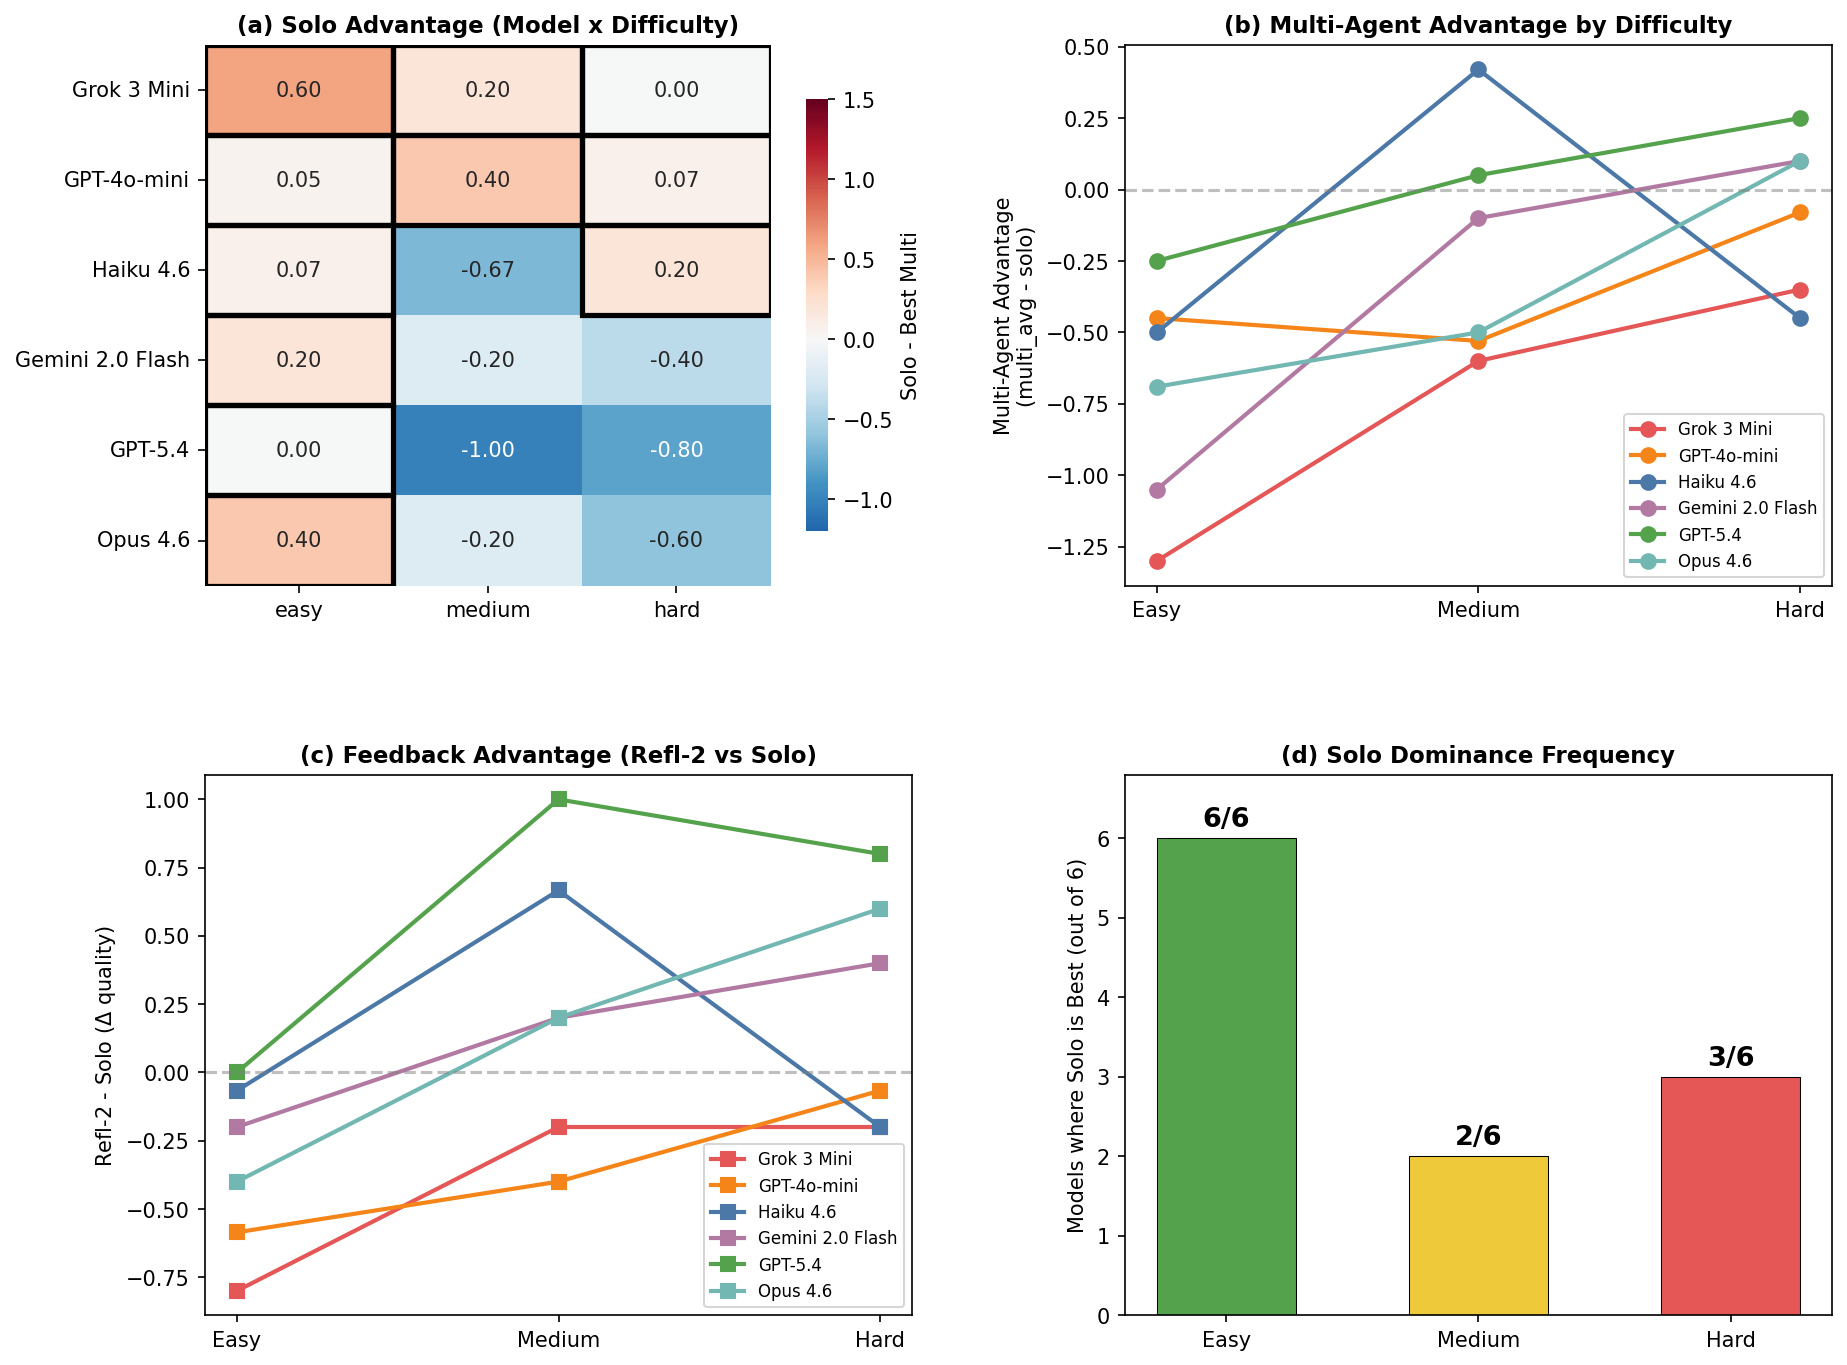
\includegraphics[width=\columnwidth]{fig10_difficulty_analysis.png}
\caption{6개 모델 난이도 $\times$ 패턴 분석. (a)~Solo 우위 히트맵: 양수(적색) = solo 우수; 검은 테두리 = solo 최적 패턴. (b)~모델별 난이도에 따른 멀티 에이전트 이점. (c)~Refl-2 vs Solo 품질 차이---역U자는 Haiku에서만 출현. (d)~모델별 Solo 우위 빈도.}
\label{fig:difficulty}
\end{figure}

%=========================================================================
\section{논의}
\label{sec:discussion}
%=========================================================================

\subsection{토폴로지 인식 종료를 위한 설계 가이드라인}

실험 결과에 기반하여, 멀티 에이전트 LLM 시스템 배포 실무자를 위한 실용적 가이드라인을 제안한다:

\paragraph{가이드라인 1: 종료 전략을 토폴로지 범주에 맞춰라.}
\begin{itemize}
  \item \emph{고정 순차 (범주 A)}: 에이전트 수 보정 max\_messages를 사용. $n$개 에이전트에 대해 max\_messages $= 2n$을 기준선으로 설정.
  \item \emph{중앙 집중형 라우팅 (범주 B1)}: 턴 예산에 조정자 오버헤드를 반영. 준선형 스케일링 (sel4/sel3 = 1.48배).
  \item \emph{탈중앙 핸드오프 (범주 B2)}: 턴 폭증을 방지하는 핸드오프 깊이 제한을 설정. 초선형 스케일링 위험 (swm4/swm3 = 3.17배).
  \item \emph{구조화 피드백 (범주 C)}: 고정 턴 한도 대신 수렴 신호를 모니터링.
  \item \emph{복합 (범주 D)}: 단계별 종료를 독립 적용.
\end{itemize}

\paragraph{가이드라인 2: 입력 토큰 증가를 예산에 반영하라.}
라운드 로빈 토폴로지에서 입력 토큰은 턴 수에 초선형으로 증가한다. $n$-에이전트 팀의 $k$라운드에 대해 예상 입력 토큰은 $O(n \cdot k \cdot \bar{L})$로 확장된다.

\paragraph{가이드라인 3: 과제-토폴로지 상호작용을 고려하라.}
단일 토폴로지 내에서 과제 범주에 따른 토큰 소비의 2.2배 변동을 보인다.

\paragraph{가이드라인 4: 키워드 신뢰도 $<$50\%인 토폴로지에 하이브리드 키워드+$\Delta U$ 종료를 배치하라.}
키워드 신뢰도가 낮은 토폴로지(예: swm4: 28\%)에 하이브리드 키워드+$\Delta U$ ($\lambda \geq 0.1$)를 적용하여 최대 78\%의 낭비 토큰을 회수한다. 신뢰도 높은 토폴로지(sel, pipe, refl)에는 모니터링 오버헤드를 피하기 위해 키워드 단독을 유지한다.

\paragraph{가이드라인 5: 토폴로지 복잡도를 과제 난이도에 맞춰라.}
비용 예측 분석은 \texttt{agent\_count $\times$ max\_messages}가 주요 비용 동인임을 보인다. 실험 07의 6개 모델 743회 실행은 난이도와 모델 능력이 최적 토폴로지를 공동 결정함을 밝힌다:
\begin{itemize}
  \item \emph{쉬운 과제}: Solo가 5/6 모델에서 충분하다 (6개 모델 평균 품질=4.85).
  \item \emph{보통/어려운 과제}: 능력 있는 기반 모델(Haiku, GPT-5.4)에서 피드백 협업(Refl-2)이 이점을 보이나 ($d$=1.26--1.83), 약한 모델에서는 Solo가 여전히 우수하다.
\end{itemize}

\subsection{멀티 에이전트 시스템 설계에의 시사점}

\textbf{세 가지 비자명 발견이 기존 멀티 에이전트 통념에 도전한다.} 첫째, 3-에이전트 탈중앙 스웜(swm3, 4,196 토큰)이 2-에이전트 순차 체인(rr2, 4,759 토큰)보다 저렴하다---\emph{더 많은 에이전트가 더 적은 비용}을 내는 비용 역전이다. 둘째, 품질 개선 메커니즘으로 널리 옹호되는 토론이 첫 라운드 이후 단조 품질 \emph{하락}을 보인다($3.8 \to 3.4 \to 3.3$). 셋째, 단순한 TERMINATE 키워드가 7/8 토폴로지에서 거의 최적이어서, 대부분의 배포에서 정교한 적응적 종료가 불필요하다---상당한 실용적 가치를 지닌 ``부정적 결과''이다.

\textbf{토폴로지 선택은 비용-품질 레버.} 토폴로지 선택은 단순한 아키텍처 결정이 아니라 비용-품질 파레토 프론티어에 대한 직접적 레버이다.

\textbf{조정자 오버헤드 세금 vs 핸드오프 폭증.} 중앙 집중형 라우팅 (범주 B1)은 ``조정자 세금''을 지불한다---각 라우팅 결정이 출력 토큰을 직접 생성하지 않는 LLM 호출을 요구한다. 반면 탈중앙 핸드오프 (범주 B2)는 조정자 세금이 없으나, 에이전트 수 증가 시 턴 폭증이 발생한다.

\textbf{출력에서의 협력적 증폭.} 에이전트별 기여 감소의 예상과 달리, LLM 호출당 출력 토큰이 팀 규모에 따라 \emph{증가}한다: rr2=930, rr3=1,189, rr4=1,544 토큰/호출. 더 풍부한 선행 컨텍스트에 노출된 에이전트는 더 길고 상세한 응답을 생성한다. 이는 AgentDropout \citep{wang2025agentdropout}의 발견과 일맥상통하나, 다른 프레이밍을 제안한다: 문제는 에이전트가 \emph{덜} 기여하는 것이 아니라, 선행 기여를 \emph{읽는} 비용이 새로운 기여를 \emph{쓰는} 가치를 앞지르는 것이다.

\textbf{보편적 신호로서의 수렴.} 수렴 감지는 주로 토론 패턴에서 연구되었으나 \citep{hu2025when}, 전체 13개 토폴로지로의 확장은 수렴 신호가 범주 전반에 존재함을 밝힌다---단지 다르게 발현될 뿐이다.

\subsection{한계}

\begin{enumerate}
\item \textbf{6개 모델 재현.} 난이도 실험을 Haiku~4.5, Opus~4.6, GPT-4o-mini, GPT-5.4, Grok~3~Mini (오픈웨이트, Apache~2.0), Gemini-2.0-Flash에 걸쳐 재현했다 (총 743회). 쉬운 과제에서 Solo 우위는 5/6 모델에서 확인되며, 보통/어려운 과제에서 피드백 이점은 능력 의존적. GPT-4o-mini 비용 순서 재현 ($\rho$=0.762, $p$=0.028)으로 토폴로지 상대 역학이 모델 불변임을 확인했다. 추가 오픈웨이트 패밀리(Llama, Mistral)로의 확장이 필요하다.

\item \textbf{과제 모음 설계 범위.} 25개 과제 모음이 9개 도메인과 4개 인지 유형을 포괄하지만 개방형 생성 과제에 집중한다. 표준 벤치마크(MMLU, HumanEval 등)는 단일 정답 평가에 설계되어 종료 분석의 핵심인 턴별 품질 궤적 추적이 불가능하다; 본 과제 모음은 이 목적에 맞게 설계되었다.

\item \textbf{품질 추정기 신뢰도.} 4개 제공자의 6개 모델(오픈웨이트 1개 포함) 교차검증 ($\kappa_w$=0.244--0.507, 4개 모델 $\geq$ moderate)으로 양방향 편향(엄격: Haiku +0.91, GPT-5.4 +0.69, Opus +0.57; 관대: Gemini $-$0.82, Grok $-$0.60)을 확인; 단일 전문 평가자. 다만 6개 교차검증 모델 전체에서 순위 일치가 유의하며 ($r$=0.43--0.66, 모두 $p<$0.01; 4개 모델 $\kappa_w \geq 0.40$), 양방향 편향 패턴(3개 관대, 3개 엄격)은 체계적 평가자 편향의 부재를 시사한다.

\item \textbf{인프라 교란 변수.} 28K 문자 프롬프트 절단 한계는 SDK 구현에 특유하다.

\item \textbf{비용 모델 단순화.} 토큰 수를 비용의 대리 변수로 사용하여, 지연 시간 민감 응용을 무시한다.

\item \textbf{하이브리드 종료의 제한적 검증.} 키워드+$\Delta U$ 하이브리드 전략을 6개 대표 패턴(swm4, debate3, rr3, sel3, refl2, pipe)에서 검증하였다. 추가 패턴으로의 확장이 필요하다.

\item \textbf{단일 인간 평가자.} 인간 평가 연구가 단일 전문 평가자의 30개 층화 표본을 사용한다. 향후 최소 2인의 인간 평가자와 Cohen's $\kappa \geq 0.60$ 보고가 필요하다.

\item \textbf{신뢰 구간 부재.} 대부분의 결과 표가 평균값만 보고한다. 패턴별 표본 크기(25--60회)는 제한적이다.

\item \textbf{표본 크기.} 패턴별 $n$=25--60; 일부 표에 표준편차 미기재.

\item \textbf{$R^{2}=0.54$의 맥락.} 행동 예측 모델에서 $R^{2}>0.30$은 의미 있고 $R^{2}>0.50$은 강한 것으로 간주된다 \citep{cohen1988}. 토폴로지 특성만으로 $R^{2}=0.54$를 달성한 것은 순수 구조적 예측 변수로서 주목할 만하다.

\item \textbf{난이도 조작화.} 실험 07의 난이도 등급은 인지 요구도에 기반하며, 합리적이나 주관적인 조작화이다.
\end{enumerate}

\subsection{향후 연구}

\begin{enumerate}
\item \textbf{동적 토폴로지 전환.} 수렴 신호에 기반한 중간 실행 토폴로지 전환.
\item \textbf{학습된 종료 정책.} 강화학습 등의 학습된 정책이 대화 궤적에 기반하여 $\lambda$를 실시간 적응.
\item \textbf{교차 모델 일반화.} 오픈웨이트 모델(Llama, Mistral)로의 확장.
\item \textbf{인간 참여 종료.} 적응적 종료와 인간 피드백을 통합한 하이브리드 종료 메커니즘.
\item \textbf{대규모 팀으로의 확장.} 10+ 에이전트로 확장 시 새로운 조정 도전.
\item \textbf{강화된 비용 예측.} 과제 수준 특성(프롬프트 복잡도, 도메인 임베딩)을 통합.
\item \textbf{난이도 적응적 토폴로지 선택.} 자동화 시스템이 수신 과제를 난이도별로 분류하고 적절한 토폴로지로 라우팅.
\end{enumerate}

%=========================================================================
\section{결론}
\label{sec:conclusion}
%=========================================================================

멀티 에이전트 시스템이 추론 시간 컴퓨팅 확장의 핵심 메커니즘이 되면서, 언제 멈출지를 이해하는 것이 필수적이다. 14개 토폴로지에 걸친 2,200회 이상의 실행과 4개 제공자의 6개 모델(오픈웨이트 Grok~3~Mini 포함)을 통해 다섯 가지 핵심 결과를 확립한다. \textbf{(1)~토폴로지가 종료를 결정한다}: 조정 오버헤드가 3.3--17.4배에 걸치며, 중앙 집중형 vs 탈중앙 라우팅이 근본적으로 다른 비용 스케일링을 보인다---토폴로지 불가지적 종료 기준으로는 보이지 않는 차이다. \textbf{(2)~에이전트가 많아도 비용이 줄 수 있다}: 3-에이전트 탈중앙 스웜이 2-에이전트 체인보다 저렴하며, 에이전트 수가 항상 비용 증가를 의미한다는 직관을 뒤집는다. \textbf{(3)~단순 휴리스틱이 거의 최적이나, 완전하지는 않다}: 키워드 종료가 8개 중 7개 토폴로지에서 거의 최적이지만, 예외에 대해 하이브리드 키워드+$\Delta U$ 전략이 품질 손실 없이 78\% 토큰 절감을 달성한다. \textbf{(4)~과제 난이도가 토폴로지를 압도한다}: 6개 모델 재현(743회)으로 난이도가 패턴 선택을 지배함을 확인한다 ($\eta^{2}_{H}=0.364$); Solo가 쉬운 과제에서 5/6 모델에서 최적이며, 피드백 패턴(Refl-2)은 능력 있는 기반 모델에서만 보통/어려운 과제에서 이점을 보인다 ($d$=1.26--1.83). \textbf{(5)~교차 제공자 검증}: 4개 제공자의 6개 모델 ($\kappa_w=0.24$--$0.51$)이 평가자 독립적 발견을 확인한다. 이 결과들은 실행 가능한 설계 가이드라인을 제공한다: 종료 전략을 토폴로지에 맞추고, 보통 난이도 과제에서만 능력 있는 기반 모델에 멀티 에이전트 팀을 배치하며, 신뢰할 수 없는 토폴로지에는 $\Delta U$ 모니터링을 사용한다. 이 발견은 추론 시 컴퓨팅 예산 배분, 자동 토폴로지 선택, 실무자의 의사결정 프레임워크에 직접적 시사점을 제공한다. 재현성과 후속 연구를 위해 실험 프레임워크를 공개한다.

%=========================================================================
% 참고 문헌
%=========================================================================
\renewcommand{\refname}{참고 문헌}
\bibliographystyle{plainnat}
\bibliography{references}

%=========================================================================
\appendix
%=========================================================================

%% =====================================================================
%% 부록: 본문에서 이동한 상세 결과 표
%% =====================================================================

\section{실험 01 상세 결과}
\label{app:exp01-details}

\begin{table}[H]
\centering
\caption{단일 에이전트 베이스라인 vs 최소 멀티 에이전트 패턴}
\label{tab:solo-baseline}
{\small
\begin{tabular}{llcrrcc}
\toprule
패턴 & 범주 & 에이전트 수 & 평균 토큰 & 평균 소요(초) & 키워드\% & vs solo \\
\midrule
solo & S & 1 & 1,287 & 18.7 & 100\% & 1.00x \\
rr2  & A & 2 & 4,759 & 52.4 & --- & 3.70x \\
swm3 & B2 & 3 & 4,196 & 75.2 & --- & 3.26x \\
sel3 & B1 & 3+1 & 7,851 & 115.2 & --- & 6.10x \\
refl2 & C & 2 & 5,237 & 60.2 & --- & 4.07x \\
\bottomrule
\end{tabular}
}
\end{table}

\begin{table}[H]
\centering
\caption{범주 A 효율 지표 (성공 실행만)}
\label{tab:cat-a-efficiency}
{\small
\begin{tabular}{lrrr}
\toprule
지표 & rr2 (n=2) & rr3 (n=3) & 비율 (rr3/rr2) \\
\midrule
성공 실행      & 55/60 & 46/60 & --- \\
오류율          & 8.3\% & 23.3\% & 2.81배 \\
평균 LLM 호출  & 2.0 & 3.5 & 1.75배 \\
평균 지속시간 (초) & 52.4 & 96.6 & 1.84배 \\
평균 입력 토큰  & 1,594 & 4,132 & 2.59배 \\
평균 출력 토큰  & 3,165 & 5,989 & 1.89배 \\
평균 총 토큰    & 4,759 & 10,121 & 2.13배 \\
출력 토큰/호출  & 1,583 & 1,711 & 1.08배 \\
\bottomrule
\end{tabular}
}
\end{table}

\begin{table}[H]
\centering
\caption{3-패턴 전체 비교 (성공 실행만)}
\label{tab:cat-a-three}
{\small
\begin{tabular}{lrrrcc}
\toprule
지표 & rr2 (n=2) & rr3 (n=3) & rr4 (n=4) & rr3/rr2 & rr4/rr2 \\
\midrule
성공 실행       & 55/60 & 46/60 & 17/60 & --- & --- \\
오류율           & 8.3\% & 23.3\% & 71.7\% & 2.81배 & 8.64배 \\
평균 지속시간 (초) & 52.4 & 96.6 & 118.8 & 1.84배 & 2.27배 \\
평균 입력 토큰   & 1,594 & 4,132 & 4,274 & 2.59배 & 2.68배 \\
평균 출력 토큰   & 3,165 & 5,989 & 7,767 & 1.89배 & 2.45배 \\
평균 총 토큰     & 4,759 & 10,121 & 12,040 & 2.13배 & 2.53배 \\
출력/에이전트 턴 & 1,583 & 1,701 & 1,942 & 1.07배 & 1.23배 \\
\bottomrule
\end{tabular}
}
\end{table}

\begin{table}[H]
\centering
\caption{과제 범주 효과 (범주 A 합산)}
\label{tab:task-category-effect}
{\small
\begin{tabular}{lcrrc l}
\toprule
과제 범주 & 실행 수 & 평균 지속시간 & 평균 토큰 & 오류율 & 특성 \\
\midrule
사실형 & 30 & 66.5초 & 6,183 & 0\% & 검색 기반, 최단 \\
창의형 & 30 & 93.3초 & 8,578 & 10.0\% & 개방형, 다라운드 \\
분석형 & 30 & 82.1초 & 8,152 & 10.0\% & 구조화 추론 \\
기술형 & 19$^{*}$ & 61.9초 & 9,100 & 42.1\% & 토큰 밀집, 절단 취약 \\
\bottomrule
\end{tabular}
}

\smallskip
{\footnotesize $^{*}$기술형은 rr3 부분 완료로 인해 실행 수가 적다.}
\end{table}

\begin{table}[H]
\centering
\caption{범주 B1 (Star) 및 B2 (Mesh) 효율 지표}
\label{tab:cat-b}
{\small
\begin{tabular}{lrrrr}
\toprule
지표 & B1: Sel-3 & B1: Sel-4 & B2: Swm-3 & B2: Swm-4 \\
    & (n=3+1)   & (n=4+1)   & (n=3)     & (n=4)     \\
\midrule
성공 실행       & 60/60 & 60/60 & 60/60 & 60/60 \\
오류율           & 0\% & 0\% & 0\% & 0\% \\
평균 지속시간 (초) & 115.2 & 161.9 & 75.2 & 185.0 \\
평균 입력 토큰   & 2,076 & 2,457 & 1,364 & 6,786 \\
평균 출력 토큰   & 5,775 & 9,138 & 2,833 & 6,535 \\
평균 총 토큰     & 7,851 & 11,595 & 4,196 & 13,321 \\
평균 턴 수       & 3.5 & 4.1 & 10.2 & 25.0 \\
평균 에이전트 턴 & 2.5 & 3.1 & 9.2 & 24.0 \\
출력/에이전트 턴 & 2,114 & 2,616 & 337 & 330 \\
\bottomrule
\end{tabular}
}
\end{table}

\begin{table}[H]
\centering
\caption{전략 간 비교 (범주 A vs B)}
\label{tab:cross-ab}
{\small
\begin{tabular}{lcrrcc}
\toprule
패턴 & 에이전트 & 지속시간 (초) & 총 토큰 & vs rr3 시간 & vs rr3 토큰 \\
\midrule
rr2  & 2   & 52.4  & 4,759  & 0.54x & 0.47x \\
rr3  & 3   & 96.6  & 10,121 & 1.00x & 1.00x \\
sel3 & 3+1 & 115.2 & 7,851  & 1.19x & 0.78x \\
sel4 & 4+1 & 161.9 & 11,595 & 1.68x & 1.15x \\
swm3 & 3   & 75.2  & 4,196  & 0.78x & 0.41x \\
swm4 & 4   & 185.0 & 13,321 & 1.92x & 1.32x \\
\bottomrule
\end{tabular}
}
\end{table}

\begin{table}[H]
\centering
\caption{범주 C 효율 지표 (전체 실행 성공)}
\label{tab:cat-c}
{\small
\begin{tabular}{lrrrr}
\toprule
지표 & Refl-2 & Refl-3 & Deb-3 & Deb-4 \\
    & (n=2)  & (n=3)  & (n=3+1) & (n=4+1) \\
\midrule
성공 실행       & 60/60 & 60/60 & 60/60 & 60/60 \\
평균 지속시간 (초) & 60.2 & 120.2 & 156.6 & 180.9 \\
평균 입력 토큰   & 1,485 & 3,343 & 3,480 & 5,217 \\
평균 출력 토큰   & 3,752 & 8,752 & 5,834 & 6,420 \\
평균 총 토큰     & 5,237 & 12,095 & 9,313 & 11,637 \\
평균 턴 수       & 3.2 & 4.5 & 4.5 & 5.4 \\
평균 에이전트 턴 & 2.2 & 3.5 & 3.5 & 4.4 \\
출력/에이전트 턴 & 1,732 & 2,537 & 1,691 & 1,448 \\
\bottomrule
\end{tabular}
}
\end{table}

\begin{table}[H]
\centering
\caption{범주 D 효율 지표 (전체 실행 성공)}
\label{tab:cat-d}
{\small
\begin{tabular}{lrr}
\toprule
지표 & Pipe (5에이전트, 2단계) & MoA (3병렬+1집약) \\
\midrule
성공 실행       & 60/60 & 60/60 \\
오류율           & 0\% & 0\% \\
평균 지속시간 (초) & 129.6 & 103.0 \\
평균 입력 토큰   & 4,275 & 4,875 \\
평균 출력 토큰   & 9,581 & 17,458 \\
평균 총 토큰     & 13,856 & 22,333 \\
평균 턴 수       & 6.0 & 11.0 \\
평균 에이전트 턴 & 4.0 & 7.0 \\
출력/에이전트 턴 & 2,325 & 2,494 \\
\bottomrule
\end{tabular}
}
\end{table}

\begin{table}[H]
\centering
\caption{범주 D 과제별 총 토큰 비교}
\label{tab:cat-d-task}
{\small
\begin{tabular}{lrrc}
\toprule
과제 범주 & Pipe & MoA & MoA/Pipe \\
\midrule
사실형 & 9,930  & 15,064 & 1.52배 \\
분석형 & 12,342 & 18,598 & 1.51배 \\
창의형 & 13,929 & 17,826 & 1.28배 \\
기술형 & 19,223 & 37,844 & 1.97배 \\
\bottomrule
\end{tabular}
}
\end{table}

\begin{table}[H]
\centering
\caption{범주 간 Kruskal-Wallis 검정 (df=4, N=718)}
\label{tab:kw-cross-cat}
{\small
\begin{tabular}{lrrrl}
\toprule
지표 & $H$ & $p$-값 & $\eta^{2}_{H}$ & 효과 크기 \\
\midrule
턴 수        & 408.606 & $<$0.001 & 0.567 & 대 \\
지속 시간(초) & 70.776  & $<$0.001 & 0.094 & 중 \\
총 토큰      & 132.333 & $<$0.001 & 0.180 & 대 \\
입력 토큰    & 60.885  & $<$0.001 & 0.080 & 중 \\
출력 토큰    & 120.565 & $<$0.001 & 0.163 & 대 \\
\bottomrule
\end{tabular}
}

\smallskip
{\footnotesize 효과 크기: $\eta^{2}_{H} = (H - k + 1) / (N - k)$, $k=5$ 범주. 기준: 소=0.01, 중=0.06, 대=0.14 \citep{cohen1988}.}
\end{table}

\begin{table}[H]
\centering
\caption{총 토큰에 대한 쌍별 Mann-Whitney U 검정 (5개 범주)}
\label{tab:pairwise-mwu}
{\small
\begin{tabular}{lrrl}
\toprule
비교 & $U$ & $p$-값 & 유의 \\
\midrule
A vs B1           & 6,000  & 0.042   & 예 \\
\textbf{A vs B2}  & \textbf{7,176}  & \textbf{0.857} & \textbf{아니오} \\
A vs C            & 11,034 & $<$0.001 & 예 \\
A vs D            & 1,778  & $<$0.001 & 예 \\
\textbf{B1 vs B2} & \textbf{8,157}  & \textbf{0.075} & \textbf{아니오 (경계)} \\
B1 vs C           & 14,035 & 0.695   & 아니오 \\
B1 vs D           & 3,010  & $<$0.001 & 예 \\
\textbf{B2 vs C}  & \textbf{12,348} & \textbf{0.028} & \textbf{예} \\
B2 vs D           & 2,944  & $<$0.001 & 예 \\
C vs D            & 5,216  & $<$0.001 & 예 \\
\bottomrule
\end{tabular}
}
\end{table}

\begin{table}[H]
\centering
\caption{범주별 토큰 소비 (5개 범주)}
\label{tab:cat-token-summary}
{\small
\begin{tabular}{llrrr}
\toprule
범주 & & 중앙값 & 평균 & $N$ \\
\midrule
A  & (순차 체인)    & 7,420  & 7,898  & 118 \\
B1 & (중앙 집중/Star) & 9,197  & 9,723  & 120 \\
B2 & (분산/Mesh)     & 9,142  & 8,759  & 120 \\
C  & (피드백)        & 9,247  & 9,571  & 240 \\
D  & (복합)          & 15,865 & 18,094 & 120 \\
\bottomrule
\end{tabular}
}
\end{table}

\begin{table}[H]
\centering
\caption{범주 내 에이전트 수 효과}
\label{tab:spearman-agents}
{\small
\begin{tabular}{lrrc}
\toprule
범주 & Spearman $\rho$ (에이전트 수 vs 턴 수) & $p$-값 & $N$ \\
\midrule
A (순차 체인)  & 0.948 & $<$0.001 & 118 \\
B1 (중앙 집중) & 0.377 & $<$0.001 & 120 \\
B2 (분산)      & 0.704 & $<$0.001 & 120 \\
C (피드백)     & 0.805 & $<$0.001 & 240 \\
\bottomrule
\end{tabular}
}
\end{table}

\begin{table}[H]
\centering
\caption{도메인 $\times$ 패턴 효율 (평균 총 토큰, $\times 10^{3}$)}
\label{tab:domain-pattern}
{\footnotesize
\begin{tabular}{lrrrrrrrr}
\toprule
도메인 & rr3 & sel3 & sel4 & swm3 & swm4 & refl2 & deb3 & pipe \\
\midrule
과학     & 9.5  & 9.3  & 7.0  & 3.3  & 9.6  & 3.5  & 6.4  & 14.2 \\
CS       & 13.4 & 8.5  & 11.6 & 5.3  & 7.9  & 4.9  & 8.7  & 13.5 \\
역사     & 7.0  & 4.2  & 5.2  & 1.4  & 12.1 & 9.1  & 8.6  & 8.9  \\
철학     & 7.9  & 3.3  & 3.2  & 8.0  & 20.7 & 2.8  & 7.7  & 8.6  \\
법/정치  & 17.4 & 10.0 & 17.4 & 1.9  & 12.3 & 4.8  & 8.4  & 10.4 \\
게임     & 20.6 & 15.1 & 14.7 & 2.6  & 13.1 & 6.9  & 10.6 & 16.5 \\
공학     & 8.8  & 12.5 & 17.8 & 3.9  & 8.2  & 5.0  & 9.8  & 12.2 \\
경영     & 15.5 & 4.4  & 13.9 & 9.2  & 14.8 & 3.5  & 8.9  & 15.7 \\
의학     & 7.9  & 10.7 & 9.5  & 1.7  & 27.1 & 10.6 & 9.2  & 29.6 \\
\bottomrule
\end{tabular}
}
\end{table}

\begin{table}[H]
\centering
\caption{패턴 도메인 민감도 (도메인 간 평균 토큰의 변동계수)}
\label{tab:domain-cv}
{\small
\begin{tabular}{llrrrl}
\toprule
패턴 & 범주 & 평균 토큰 & 표준편차 & CV & 해석 \\
\midrule
debate3 & C  & 8,657  & 1,189 & 0.14 & 도메인 불변 \\
rr3     & A  & 12,005 & 4,907 & 0.41 & 중간 \\
pipe    & D  & 14,404 & 6,361 & 0.44 & 중간 \\
swm4    & B2 & 13,969 & 6,268 & 0.45 & 중간 \\
sel3    & B1 & 8,665  & 4,019 & 0.46 & 중간 \\
refl2   & C  & 5,675  & 2,666 & 0.47 & 중간 \\
sel4    & B1 & 11,131 & 5,264 & 0.47 & 중간 \\
swm3    & B2 & 4,148  & 2,795 & 0.67 & 도메인 민감 \\
\bottomrule
\end{tabular}
}
\end{table}

\section{실험 02 상세 결과}
\label{app:exp02-details}

\begin{table}[H]
\centering
\caption{품질 궤적 (실질 턴별 평균 종합 점수)}
\label{tab:quality-trajectory}
{\small
\begin{tabular}{lcccccc}
\toprule
패턴 & $t_1$ & $t_2$ & $t_3$ & $t_4$ & $t_5$ & $t_6$ \\
\midrule
rr3     & 3.9 & 4.2 & 4.5 & 4.1 & 4.1 & 4.1 \\
sel3    & 3.8 & 3.5 & 2.7 & 4.0 & 4.0 & --- \\
swm3    & 4.2 & 3.0 & 2.0 & --- & --- & --- \\
refl2   & 3.9 & 4.8 & 4.0 & 4.0 & --- & --- \\
debate3 & 3.8 & 3.4 & 3.3 & 3.3 & --- & --- \\
\bottomrule
\end{tabular}
}
\end{table}

\begin{table}[H]
\centering
\caption{차원별 분석 (최종 턴 평균)}
\label{tab:dimension-analysis}
{\small
\begin{tabular}{lccccc}
\toprule
패턴 & 정확성 & 완전성 & 일관성 & 유용성 & 종합 \\
\midrule
refl2   & 4.80 & 4.25 & 5.00 & 4.95 & 4.80 \\
rr3     & 4.50 & 3.75 & 4.25 & 4.70 & 4.45 \\
swm3    & 4.25 & 3.80 & 4.45 & 4.35 & 4.05 \\
sel3    & 3.85 & 3.15 & 3.35 & 3.80 & 3.40 \\
debate3 & 3.75 & 2.70 & 3.35 & 3.55 & 3.35 \\
\bottomrule
\end{tabular}
}
\end{table}

\begin{table}[H]
\centering
\caption{교차 모델 일치도 (Claude G-Eval vs.\ 6개 독립 모델)}
\label{tab:cross-model-agreement}
{\small
\begin{tabular}{llccccc}
\toprule
교차검증 모델 & 제공자 & $N$ & Pearson $r$ & Spearman $\rho$ & Cohen's $\kappa_w$ & $\Delta$ \\
\midrule
GPT-4o-mini      & OpenAI    & 40  & 0.434 & 0.389 & 0.244 & $-$0.93 \\
Gemini 2.0 Flash & Google    & 100 & 0.569 & 0.500 & 0.359 & $-$0.82 \\
GPT-5.4          & OpenAI    & 100 & 0.540 & 0.525 & 0.415 & $+$0.69 \\
Haiku 4.5        & Anthropic & 100 & 0.662 & 0.650 & 0.425 & $+$0.91 \\
Grok 3 Mini      & xAI       & 100 & 0.628 & 0.626 & 0.449 & $-$0.60 \\
Opus 4.6         & Anthropic & 100 & 0.632 & 0.649 & \textbf{0.507} & $+$0.57 \\
\bottomrule
\end{tabular}
}
\end{table}

\section{실험 03 상세 결과}
\label{app:exp03-details}

\begin{table}[H]
\centering
\caption{패턴별 의미적 수렴 분석 ($\theta=0.85$)}
\label{tab:semantic-convergence}
{\small
\begin{tabular}{llcccccr}
\toprule
패턴 & 범주 & $N$ & 수렴율 & 평균코사인 & 최종코사인 & 추세 & 수렴턴 \\
\midrule
rr3     & A  & 25 & 16.0\% & 0.576 & 0.690 & +0.250  & 3.0 \\
sel3    & B1 & 25 & 24.0\% & 0.403 & 0.602 & +0.397  & 3.0 \\
sel4    & B1 & 25 & 28.0\% & 0.502 & 0.661 & +0.382  & 3.6 \\
swm3    & B2 & 25 & 8.0\%  & 0.458 & 0.132 & $-$0.560 & 7.0 \\
swm4    & B2 & 25 & 16.0\% & 0.485 & 0.453 & $-$0.029 & 15.5 \\
refl2   & C  & 25 & 0.0\%  & 0.462 & 0.479 & +0.052  & N/A \\
debate3 & C  & 25 & 0.0\%  & 0.673 & 0.681 & +0.044  & N/A \\
pipe    & D  & 25 & \textbf{32.0\%} & 0.662 & 0.688 & +0.169 & 3.9 \\
\bottomrule
\end{tabular}
}
\end{table}

\begin{table}[H]
\centering
\caption{Jaccard vs 임베딩 비교}
\label{tab:jaccard-vs-embedding}
{\footnotesize
\begin{tabular}{llcccc}
\toprule
패턴 & 범주 & 평균 Jaccard & 평균 코사인 & Jaccard 수렴 ($\theta$=0.25) & 코사인 수렴 ($\theta$=0.85) \\
\midrule
rr3     & A  & 0.007 & 0.576 & 0.0\%  & 16.0\% \\
sel3    & B1 & 0.004 & 0.403 & 0.0\%  & 24.0\% \\
sel4    & B1 & 0.004 & 0.502 & 0.0\%  & 28.0\% \\
swm3    & B2 & 0.134 & 0.458 & 12.0\% & 8.0\%  \\
swm4    & B2 & 0.130 & 0.485 & 44.0\% & 16.0\% \\
refl2   & C  & 0.005 & 0.462 & 0.0\%  & 0.0\%  \\
debate3 & C  & 0.006 & 0.673 & 0.0\%  & 0.0\%  \\
pipe    & D  & 0.012 & 0.662 & 0.0\%  & 32.0\% \\
\bottomrule
\end{tabular}
}
\end{table}

\begin{table}[H]
\centering
\caption{민감도 분석 (다른 임계값에서의 수렴율)}
\label{tab:sensitivity-theta}
{\small
\begin{tabular}{llrrr}
\toprule
패턴 & 범주 & $\theta$=0.80 & $\theta$=0.85 & $\theta$=0.90 \\
\midrule
rr3     & A  & 24.0\% & 16.0\% & 8.0\% \\
sel3    & B1 & 32.0\% & 24.0\% & 16.0\% \\
sel4    & B1 & 44.0\% & 28.0\% & 12.0\% \\
swm3    & B2 & 8.0\%  & 8.0\%  & 8.0\% \\
swm4    & B2 & 24.0\% & 16.0\% & 12.0\% \\
refl2   & C  & 8.0\%  & 0.0\%  & 0.0\% \\
debate3 & C  & 12.0\% & 0.0\%  & 0.0\% \\
pipe    & D  & 36.0\% & 32.0\% & 8.0\% \\
\bottomrule
\end{tabular}
}
\end{table}

\section{실험 04 상세 결과}
\label{app:exp04-details}

\begin{table}[H]
\centering
\caption{종료 모드 분포 (v1, 780회)}
\label{tab:termination-modes}
{\small
\begin{tabular}{llcrrr}
\toprule
패턴 & 범주 & $N$ & 키워드\% & MaxMsg\% & 오류\% \\
\midrule
rr2     & A  & 60 & 91.7\%  & 0.0\%   & 8.3\% \\
rr3     & A  & 60 & 76.7\%  & 0.0\%   & 23.3\% \\
rr4     & A  & 60 & 28.3\%  & 0.0\%   & 71.7\% \\
sel3    & B1 & 60 & 100.0\% & 0.0\%   & 0.0\% \\
sel4    & B1 & 60 & 100.0\% & 0.0\%   & 0.0\% \\
swm3    & B2 & 60 & 78.3\%  & 21.7\%  & 0.0\% \\
swm4    & B2 & 60 & 28.3\%  & 71.7\%  & 0.0\% \\
refl2   & C  & 60 & 100.0\% & 0.0\%   & 0.0\% \\
debate3 & C  & 60 & 100.0\% & 0.0\%   & 0.0\% \\
pipe    & D  & 60 & 100.0\% & 0.0\%   & 0.0\% \\
moa     & D  & 60 & 0.0\%   & 100.0\% & 0.0\% \\
\bottomrule
\end{tabular}
}
\end{table}

\begin{table}[H]
\centering
\caption{v1 과제 도메인별 오류 분포 (범주 A만)}
\label{tab:error-by-domain}
{\small
\begin{tabular}{lcccc}
\toprule
패턴 & 사실형 & 분석형 & 창의형 & 기술형 \\
\midrule
rr2 & 0/15 (0\%) & 0/15 (0\%) & 0/15 (0\%) & 5/15 (33.3\%) \\
rr3 & 0/15 (0\%) & 3/15 (20\%) & 3/15 (20\%) & 8/15 (53.3\%) \\
rr4 & 0/15 (0\%) & 15/15 (100\%) & 13/15 (86.7\%) & 15/15 (100\%) \\
\bottomrule
\end{tabular}
}
\end{table}

\section{실험 05 상세 결과}
\label{app:exp05-details}

\begin{table}[H]
\centering
\caption{한계 효용 수렴 분석 ($\lambda=0.1$)}
\label{tab:marginal-utility}
{\small
\begin{tabular}{llccccccc}
\toprule
패턴 & 범주 & $t_{\Delta U \leq 0}$ & $t_{\text{opt}}$ & $t_{\text{act}}$ & $Q_{\text{opt}}$ & $Q_{\text{act}}$ & $Q_{\text{loss}}$ & Regret \\
\midrule
swm3    & B2 & \textbf{1.1} & 1.0 & 1.2 & 4.15 & 4.05 & 0.10 & 0.2 \\
refl2   & C  & 2.0          & 1.7 & 2.3 & 4.80 & 4.80 & \textbf{0.00} & 0.6 \\
sel3    & B1 & 2.0          & 1.1 & 2.8 & 3.90 & 3.40 & 0.50 & 1.6 \\
debate3 & C  & 2.2          & 1.3 & 3.3 & 4.00 & 3.35 & 0.65 & 2.0 \\
rr3     & A  & \textbf{2.4} & 1.6 & 4.2 & 4.50 & 4.45 & 0.05 & 2.6 \\
\bottomrule
\end{tabular}
}
\end{table}

\begin{table}[H]
\centering
\caption{$\lambda$ 민감도 분석}
\label{tab:lambda-sensitivity}
{\small
\begin{tabular}{cccc}
\toprule
$\lambda$ & 평균 $t_{\Delta U \leq 0}$ & 평균 Regret & 평균 $Q_{\text{loss}}$ \\
\midrule
0.00 & 1.9 & 1.4 & 0.260 \\
0.05 & 1.9 & 1.4 & 0.260 \\
0.10 & 1.9 & 1.4 & 0.260 \\
0.20 & 1.9 & 1.4 & 0.260 \\
0.50 & 1.8 & 1.4 & 0.260 \\
\bottomrule
\end{tabular}
}

\smallskip
{\footnotesize 참고: Regret과 $Q_{\text{loss}}$가 $\lambda$에 불변인 이유는 이 지표들이 베이스라인 행동을 측정하기 때문이다. $\lambda$에 의존하는 것은 오직 $t_{\Delta U \leq 0}$뿐이다.}
\end{table}

\begin{table}[H]
\centering
\caption{Adaptive vs Baseline 비교}
\label{tab:adaptive-vs-baseline}
{\small
\begin{tabular}{llrrrrrr}
\toprule
패턴 & 범주 & BL 턴 & AD 턴 & 턴 $\Delta$\% & BL 토큰 & AD 토큰 & 토큰 $\Delta$\% \\
\midrule
rr3     & A  & 4.6  & 5.5  & +19\%  & 11,546  & 15,278  & +32\% \\
sel3    & B1 & 3.7  & 4.7  & +27\%  & 7,901   & 12,840  & +63\% \\
sel4    & B1 & 4.3  & 5.4  & +26\%  & 11,136  & 16,315  & +47\% \\
swm3    & B2 & 9.6  & 8.2  & $-$15\% & 3,223  & 9,818   & +205\% \\
swm4    & B2 & 25.6 & 9.1  & \textbf{$-$65\%} & 15,327 & 4,656 & \textbf{$-$70\%} \\
refl2   & C  & 3.3  & 6.4  & +92\%  & 5,509   & 19,693  & +258\% \\
debate3 & C  & 4.4  & 4.6  & +5\%   & 9,042   & 9,752   & +8\% \\
pipe    & D  & 5.8  & 5.8  & +1\%   & 10,853  & 12,092  & +11\% \\
\bottomrule
\end{tabular}
}
\end{table}

\begin{table}[H]
\centering
\caption{$\lambda$ 민감도 (패턴 평균)}
\label{tab:lambda-pattern-avg}
{\small
\begin{tabular}{crrr}
\toprule
$\lambda$ & 평균 턴 $\Delta$\% & 평균 토큰 $\Delta$\% & $N$ \\
\midrule
0.00 & +10\%  & +131\% & 200 \\
0.10 & $-$33\% & $-$13\% & 200 \\
0.50 & $-$34\% & $-$13\% & 200 \\
\bottomrule
\end{tabular}
}
\end{table}

\section{교차 모델 검증 상세}
\label{app:cross-model-details}

\begin{table}[H]
\centering
\caption{교차 모델 비교 (Claude Haiku 4.5 vs.\ GPT-4o-mini)}
\label{tab:cross-model-tokens}
{\small
\begin{tabular}{lrrrrrrr}
\toprule
패턴 & Claude 토큰 & GPT 토큰 & 비율 & Claude 턴 & GPT 턴 & Claude KW\% & GPT KW\% \\
\midrule
solo  & 1,287  & 697    & 0.54x & 2.0  & 2.0  & 100\% & 100\% \\
rr3   & 10,121 & 14,325 & 1.42x & 4.5  & 6.2  & 100\% & 80\% \\
sel3  & 7,851  & 3,598  & 0.46x & 3.5  & 3.5  & 100\% & 100\% \\
swm3  & 4,196  & 3,203  & 0.76x & 10.2 & 10.0 & 78\%  & 72\% \\
refl2 & 5,237  & 5,105  & 0.97x & 3.2  & 4.0  & 100\% & 92\% \\
\bottomrule
\end{tabular}
}
\end{table}

\begin{table}[H]
\centering
\caption{패턴별 비용 순위 비교}
\label{tab:cross-model-rank}
{\small
\begin{tabular}{lccrrrl}
\toprule
패턴 & Claude 순위 & GPT 순위 & Claude 토큰 & GPT 토큰 & 비율 & 방향 \\
\midrule
Solo  & 1 & 1 & 1,287  & 697    & 1.85x & Claude 고비용 \\
Swm-3 & 2 & 2 & 4,196  & 3,203  & 1.31x & Claude 고비용 \\
Refl-2 & 3 & 4 & 5,237 & 5,105  & 1.03x & 거의 동일 \\
Sel-3 & 4 & 3 & 7,851  & 3,598  & 2.18x & Claude 고비용 \\
RR-3  & 5 & 5 & 10,121 & 14,325 & 0.71x & GPT 고비용 \\
\bottomrule
\end{tabular}
}

\smallskip
{\footnotesize 주: 순위 역전(refl2$\leftrightarrow$sel3)은 중간 구간에서만 발생. 양 극단(solo 최저, rr3 최고)은 두 모델에서 보존.}
\end{table}

\section{실험 06 상세 결과}
\label{app:exp06-details}

\begin{table}[H]
\centering
\caption{비용 예측 교차 검증 결과 (5-fold CV)}
\label{tab:cost-prediction-cv}
{\small
\begin{tabular}{llcc}
\toprule
타겟 & 최적 모델 & $R^{2}$ (평균$\pm$std) & MAE \\
\midrule
총 토큰     & RandomForest & 0.54 $\pm$ 0.06 & 3,440 \\
지속 시간 (초) & RandomForest & 0.46 $\pm$ 0.04 & 34.8 \\
턴 수       & RandomForest & 0.28 $\pm$ 0.09 & 3.0 \\
\bottomrule
\end{tabular}
}
\end{table}

\begin{table}[H]
\centering
\caption{특성 중요도 (Random Forest, 총 토큰 타겟)}
\label{tab:feature-importance}
{\small
\begin{tabular}{lrl}
\toprule
특성 & RF 중요도 & 해석 \\
\midrule
task\_technical     & 0.273 & 기술형 과제가 최다 토큰 소비 \\
pat\_D (복합)       & 0.174 & 다단계 패턴이 본질적으로 고비용 \\
agents\_x\_maxmsg   & 0.158 & 상호작용 항이 스케일링 포착 \\
max\_messages       & 0.143 & 메시지 예산 $\uparrow$ $\to$ 토큰 $\uparrow$ \\
agent\_count        & 0.133 & 에이전트 수 $\uparrow$ $\to$ 통신 $\uparrow$ \\
pat\_C (피드백)     & 0.051 & 피드백 루프 = 중간 오버헤드 \\
\bottomrule
\end{tabular}
}
\end{table}

\section{실험 07 상세 결과}
\label{app:exp07-details}

\begin{table}[H]
\centering
\caption{추천 매트릭스}
\label{tab:recommendation-matrix}
{\small
\begin{tabular}{lclcr}
\toprule
난이도 & 최고 품질 & 점수 & 최고 효율 (Q/kT) & 토큰 범위 \\
\midrule
쉬움   & Solo   & 4.82 & Solo & 491--11,200 \\
보통   & Refl-2 & 3.64 & Solo & 1,032--15,752 \\
어려움 & Refl-2 & 3.20 & Solo & 5,680--28,877 \\
\bottomrule
\end{tabular}
}
\end{table}

%% =====================================================================
%% 기존 부록
%% =====================================================================

\section{과제 모음}
\label{app:task-suite}

\begin{table}[H]
\centering
\caption{전체 과제 모음 (v2, 25개, 9개 도메인)}
\label{tab:task-suite}
{\footnotesize
\begin{tabular}{lllll}
\toprule
ID & 도메인 & 인지유형 & 난이도 & 과제 설명 \\
\midrule
sci\_01  & 과학    & 사실형 & 중 & 열역학 3법칙과 공학적 시사점 설명 \\
sci\_02  & 과학    & 분석형 & 중 & 광합성 경로 비교 (C3/C4/CAM) \\
sci\_03  & 과학    & 창의형 & 상 & 암흑물질 검출 실험 3가지 제안 \\
cs\_01   & CS      & 사실형 & 중 & TCP/IP 프로토콜 스택 계층과 데이터 흐름 \\
cs\_02   & CS      & 기술형 & 중 & O(1) get/put LRU 캐시 구현 \\
cs\_03   & CS      & 분석형 & 중 & 마이크로서비스 vs 모놀리식 비교 \\
hist\_01 & 역사    & 사실형 & 중 & 1차 세계대전의 원인 분석 \\
hist\_02 & 역사    & 분석형 & 상 & 로마/대영 제국 쇠퇴 비교 \\
hist\_03 & 역사    & 창의형 & 상 & 대안 역사: 인쇄술이 송나라에서? \\
phil\_01 & 철학    & 사실형 & 중 & 칸트 정언명령 vs 밀 공리주의 \\
phil\_02 & 철학    & 분석형 & 중 & 트롤리 문제의 윤리적 분석 \\
phil\_03 & 철학    & 창의형 & 상 & AI 마인드 업로딩 사고실험 \\
law\_01  & 법/정치 & 사실형 & 중 & 삼권분립 대통령제 vs 의원내각제 \\
law\_02  & 법/정치 & 분석형 & 상 & AI 저작권법 국제 비교 \\
law\_03  & 법/정치 & 창의형 & 상 & 자율주행차 규제 정책 초안 \\
game\_01 & 게임    & 사실형 & 중 & 피드백 루프, 플로우, MDA 프레임워크 \\
game\_02 & 게임    & 기술형 & 상 & ELO/Glicko 매치메이킹 설계 \\
game\_03 & 게임    & 창의형 & 상 & 양자 컴퓨팅 퍼즐 게임 컨셉 \\
eng\_01  & 공학    & 사실형 & 중 & 교량 구조 하중 분석 \\
eng\_02  & 공학    & 기술형 & 상 & 20만 인구 수처리장 설계 \\
eng\_03  & 공학    & 분석형 & 중 & 전통 vs 3D 프린팅 건설 비교 \\
biz\_01  & 경영    & 창의형 & 상 & AI K-12 맞춤 교육 스타트업 \\
biz\_02  & 경영    & 분석형 & 중 & VC 투자 vs 부트스트래핑 비교 \\
biz\_03  & 경영    & 분석형 & 상 & 동남아 EV 시장 진입 전략 \\
med\_01  & 의학    & 분석형 & 상 & mRNA vs 단백질 서브유닛 백신 비교 \\
\bottomrule
\end{tabular}
}
\end{table}

과제는 9개 도메인 $\times$ 4개 인지유형으로 구성되며, 각 도메인에서 3개(의학 1개) 과제를 포함한다.

\section{패턴 구현 세부사항}
\label{app:pattern-impl}

13개 패턴 모두 패턴 식별자를 구성된 팀 인스턴스로 매핑하는 TeamFactory 추상화를 통해 AutoGen 프레임워크 내에서 구현된다. 각 패턴은 다음을 공유한다:
\begin{itemize}
  \item 기반 모델: Claude Haiku 4.5 (ClaudeCLIChatCompletionClient 경유)
  \item 토큰 추적: \texttt{models\_usage} 통한 호출별 프롬프트 및 완성 토큰 수
  \item 종료: TERMINATE 키워드 감지 + max\_messages 안전 상한 (25)
  \item 체크포인트: 내결함성을 위한 패턴별 결과 저장
\end{itemize}

\section{통계적 변동성}
\label{app:variability}

모든 지표는 실험 01의 v2 데이터셋(패턴당 $n=25$)과 실험 02(패턴당 $n=40$)에서 산출. 95\% 신뢰구간은 자유도 $n-1$의 $t$-분포 사용.

\begin{table}[H]
\centering
\caption{실험 01 효율 통계 (패턴당 $n=25$)}
\label{tab:c1-exp01-stats}
{\footnotesize
\begin{tabular}{llrrrrrr}
\toprule
패턴 & 범주 & 토큰 평균 & $\pm$std & 95\% CI & 시간 평균(초) & $\pm$std & 턴 평균 \\
\midrule
debate3 & C  & 8,657  & $\pm$2,501  & [7,625; 9,690]   & 121.6 & $\pm$26.2  & 3.6 \\
pipe    & D  & 13,186 & $\pm$5,828  & [10,780; 15,592] & 128.3 & $\pm$58.3  & 4.0 \\
refl2   & C  & 5,281  & $\pm$3,315  & [3,913; 6,649]   & 53.1  & $\pm$29.0  & 2.2 \\
rr3     & A  & 12,332 & $\pm$10,148 & [8,143; 16,521]  & 111.4 & $\pm$90.4  & 3.6 \\
sel3    & B1 & 8,502  & $\pm$5,243  & [6,338; 10,666]  & 95.6  & $\pm$42.4  & 2.7 \\
sel4    & B1 & 11,264 & $\pm$6,428  & [8,610; 13,917]  & 124.5 & $\pm$62.9  & 3.2 \\
swm3    & B2 & 4,341  & $\pm$5,646  & [2,011; 6,672]   & 45.4  & $\pm$30.9  & 7.8 \\
swm4    & B2 & 12,921 & $\pm$6,214  & [10,355; 15,486] & 148.6 & $\pm$39.1  & 25.1 \\
\bottomrule
\end{tabular}
}

\smallskip
{\footnotesize 주: swm3의 높은 토큰 std ($\pm$5,646, 평균 4,341 대비 CV=1.30)는 스웜 행동의 이중 모드적 특성을 반영한다.}
\end{table}

\begin{table}[H]
\centering
\caption{실험 02 품질 통계 (패턴당 $n=40$)}
\label{tab:c2-exp02-stats}
{\footnotesize
\begin{tabular}{llrrrrrr}
\toprule
패턴 & 범주 & 품질 평균 & $\pm$std & 95\% CI & 토큰 평균 & $\pm$std & 95\% CI \\
\midrule
refl2   & C  & 4.80 & $\pm$0.41 & [4.67; 4.93]    & 7,186  & $\pm$11,272 & [3,606; 10,766] \\
rr3     & A  & 4.45 & $\pm$0.50 & [4.29; 4.61]    & 13,949 & $\pm$8,539  & [11,237; 16,661] \\
swm3    & B2 & 3.77 & $\pm$1.25 & [3.38; 4.17]    & 7,882  & $\pm$12,447 & [3,928; 11,836] \\
sel3    & B1 & 3.40 & $\pm$1.08 & [3.06; 3.74]    & 8,646  & $\pm$6,887  & [6,458; 10,834] \\
debate3 & C  & 3.35 & $\pm$0.80 & [3.10; 3.60]    & 8,887  & $\pm$2,457  & [8,106; 9,667] \\
\bottomrule
\end{tabular}
}
\end{table}

\begin{table}[H]
\centering
\caption{실험 05 적응적 종료 통계 (패턴당 $n=100$)}
\label{tab:c3-exp05-stats}
{\footnotesize
\begin{tabular}{llrrrrrr}
\toprule
패턴 & 범주 & 토큰 평균 & $\pm$std & 95\% CI & 시간 평균(초) & $\pm$std & 턴 평균 \\
\midrule
debate3 & C  & 9,575  & $\pm$4,931  & [8,596; 10,553]  & 119.3 & $\pm$63.1  & 3.6 \\
pipe    & D  & 11,783 & $\pm$5,982  & [10,596; 12,969] & 118.4 & $\pm$58.5  & 3.8 \\
refl2   & C  & 16,147 & $\pm$24,176 & [11,350; 20,943] & 170.3 & $\pm$262.6 & 4.6 \\
rr3     & A  & 14,345 & $\pm$14,162 & [11,535; 17,155] & 136.6 & $\pm$136.3 & 4.2 \\
sel3    & B1 & 11,606 & $\pm$7,797  & [10,059; 13,153] & 153.0 & $\pm$95.2  & 3.5 \\
sel4    & B1 & 15,020 & $\pm$13,180 & [12,405; 17,635] & 174.4 & $\pm$159.4 & 4.1 \\
swm3    & B2 & 8,169  & $\pm$9,906  & [6,204; 10,134]  & 96.6  & $\pm$98.6  & 7.5 \\
swm4    & B2 & 7,324  & $\pm$7,542  & [5,827; 8,820]   & 70.3  & $\pm$47.0  & 12.2 \\
\bottomrule
\end{tabular}
}
\end{table}

\section{압축 발견 요약}
\label{app:compressed}

본문의 47개 개별 발견을 17개 핵심 발견으로 정리한다.

\begin{table}[H]
\centering
\caption{압축 발견 요약}
\label{tab:compressed-findings}
{\footnotesize
\begin{tabular}{clll}
\toprule
\# & 핵심 발견 & 원본 & 절 \\
\midrule
C1  & 멀티 에이전트 조정은 3.3--17.4배 토큰 오버헤드; 비용 준선형, 오류율 초선형 & F1--5 & 4.1.1 \\
C2  & 중앙(B1)/분산(B2) 라우팅은 다른 스케일링: B1 준선형, B2 초선형 & F6--8 & 4.1.2 \\
C3  & swm3가 최고 토큰 효율, rr2 능가; 라우팅 전략이 에이전트 수 지배 & F8 & 4.1.2 \\
C4  & 반영/토론 반대 스케일링; 동일 수에서 반영 빠르나 토론 저렴 & F9--12 & 4.1.3 \\
C5  & 복합 패턴 가장 비싸나 최고 출력 밀도 & F13--15 & 4.1.4 \\
C6  & 새 비용 계층: A $\approx$ B2 $<$ B1 $\approx$ C $\ll$ D & F16--18 & 4.1.5 \\
C7  & debate3만 도메인 불변; 과제 복잡도가 비용 2배 증폭 & F19--21 & 4.1.6 \\
C8  & 세 품질 궤적: 고원(rr3), 정점(refl2), 하락(debate3) & F22 & 4.2 \\
C9  & 종료 후회 13배 차이; 반성 최고 품질+제로 손실 & F23--24 & 4.2 \\
C10 & 의미 수렴이 표면 지표와 다른 순위; 피드백 비수렴 & F25--27 & 4.3 \\
C11 & 세 종료 실패 모드; 사실형 면역, 기술형 취약 & F28--30 & 4.4 \\
C12 & $\Delta U$ 모든 토폴로지에서 1.1--2.4턴 내 수렴; $\lambda$ 비민감 & F31--32 & 4.5 \\
C13 & 적응적 종료 이점은 토폴로지 의존; swm4에서만 $-$70\% & F33--35 & 4.5 \\
C14 & $\Delta U$는 키워드 보완이지 대체 아님 & F36 & 4.5 \\
C15 & 토폴로지 동역학 모델 불변 ($\rho$=0.900) & F37--39 & 4.6 \\
C16 & 토폴로지 특성이 54\% 예측; agents$\times$maxmsg 최상위 & F40--42 & 4.7 \\
C17 & 난이도 지배 (6개 모델 재현, $\eta^{2}_{H}$=0.364); solo 쉬움 5/6 모델, 능력 조건부 refl2 보통/어려움 & F43--47 & 4.8 \\
\bottomrule
\end{tabular}
}
\end{table}

\end{document}
